\chapter[The post-predicate position in Turkish in contact]{The post-predicate position in Turkish in contact with German and/or Kurmanji}\label{chap:key:5}

This chapter aims to establish whether the word order in the Turkish varieties is undergoing change, with a specific focus on the post-predicate domain, and if so, what the source of the change is.

Turkish is one of the most vital heritage languages and has been extensively studied, particularly in the context of Germany. However, several important factors have often been overlooked. This study will address these gaps, as outlined below. To gain a deeper understanding of the source of change, this study analyzes post-predicate structures in Turkish across four groups: two Turkish heritage speaker groups in Germany—Turkish-German bilinguals and Turkish-Kurmanji-German trilinguals—and two majority Turkish speaker groups in Turkey—Turkish-Kurmanji bilinguals and Turkish monolinguals. Examining Turkish within these groups makes it possible to investigate the use of the post-predicate position: (1) in mono-, bi-, and trilingual speakers in contexts where Turkish holds different societal statuses, either as a heritage or majority language, (2) in different contact situations, where the intensity of contact differs based on factors such as duration and the number of speakers in the community, (3) in Turkish in contact with different languages, namely Kurmanji and/or German.

Heritage languages are often compared to their monolingual counterparts. In the present study, the inclusion of a Turkish-Kurmanji bilingual group allows for the analysis of a scenario in which Turkish is spoken by bilinguals as a majority language rather than as a heritage language. This shift enables a focus on the societal status of the investigated language rather than using monolinguals as the baseline for comparison. By making this distinction, the study can more clearly separate the effects of bilingualism from those of societal status. Moreover, including this group can also provide insights into the intensity of contact between the languages and its effects on language change: while the contact between Turkish and Kurmanji started before the Ottoman Empire times and continued more intensively after the proclamation of the Turkish Republic (\citealt{Yagmur2001}), the contact between Kurmanji and German in Germany started in the second half of the 20\textsuperscript{th} century with the arrival of guest workers to Germany (\citealt{GhaderiAlmstadt2023}). Additionally, incorporating a Turkish-Kurmanji-German trilingual group is important, as many Turkish heritage speakers in Germany also speak Kurmanji. Currently, there are only a few studies that focus on trilingual speakers.

Furthermore, the study includes two contact languages, German and Kurmanji. In terms of word order, Turkish is an SOV language, but it employs the post-predicate position for background information, particularly in informal situations \citep{Schroeder1995}. German as the contact language in Germany is also SOV but with V2 features in main declarative clauses with a finite main verb and in wh- questions \citep{Muller2023}. As for Kurmanji, it is an SOV language that systematically places goal arguments in the post-predicate position \citep{Haig2018}.

At the same time, there are also overlaps in some factors that influence the employment of the post-predicate position. For instance, \citet{Asadpour2021} claims that information structure also plays a role in the employment of the post-predicate position in Mukri Kurdish spoken in Iran. If information structure has a similar effect on the word order in Kurmanji spoken in Turkey, it would highlight an overlapping factor—information structure—for the employment of the post-predicate position in Kurmanji and Turkish.

Furthermore, a shared factor for the employment of the post-predicate position in Turkish and German is mode and formality: placing constituents in the post-field for German and the post-predicate position for Turkish is said to occur more frequently in the spoken mode compared to the written mode and in the informal language compared to the formal ones (\citealt{Roelcke1997}, \citealt{Tsehaye2023} -- for German, \citealt{Erguvanli1984}, \citealt{Schroeder1995} -- for Turkish). Concerning Kurmanji, the influence of formality and mode on its word order has not been attested, but some studies show that these two variables have an effect on the employment of the post-predicate position in Persian, which shares syntactic features with other West Iranian languages (\citealt{Frommer1981}, \citealt{Haig_post-predicate_EtAl2024-1}). Thus, the combination of similarities and differences in the factors that influence the employment of the post-predicate position across Turkish, Kurmanji, and German renders the investigated topic particularly intriguing for examination.

Finally, an important factor that has not been widely considered in heritage language research is register. This study investigates the use of the post-predicate position across various communicative situations, highlighting the significance of including formality and mode in the analysis. As discussed in Chapter 3, the post-predicate position in Turkish is strongly associated with informal and spoken registers, while being more restricted in formal communicative situations.

Heritage speakers typically acquire their heritage language from birth and become immersed in the majority language upon entering school. Hence, these languages are used in different situational-functional contexts: the heritage language is primarily spoken at home in informal settings, while the majority language is used across both formal and informal settings. Much previous research often did not account for such register difference, sometimes even comparing heritage language use in informal settings to monolingual productions in formal settings—resulting in a comparison that unfairly disadvantages bilinguals. A recent study by \citet{WieseEtAl2022} emphasizes the importance of accounting for register in linguistic studies, demonstrating that noncanonical features found in heritage languages also appear in the informal speech of monolinguals. Therefore, analyzing the occurrence of noncanonical constructions in a heritage language through the lens of different communicative situations is essential.

Taking the recent developments in the field into account, this study aims to explore the factors that drive differences between heritage and majority language varieties by entertaining such factors as CLI, internal dynamics in the languages, and particularly the role of register.

The chapter will begin by analyzing the frequency distribution of post-predicate structures across various Turkish varieties (\sectref{sec:key:5.1}), followed by an exploration of their usage in different communicative situations (\sectref{sec:key:5.2}). Next, the chapter will investigate the composition of post-predicate structures, focusing on factors such as weight, type, and semantic role (\sectref{sec:key:5.3}). Finally, the discussion will turn to the information status of the post-predicate elements (\sectref{sec:key:5.4}).

\section[Frequency distributions  in heritage and majority Turkish]{Frequency distributions of post-predicate constituents in heritage and majority Turkish}\label{sec:key:5.1}

The analysis begins with an overview of the frequency distribution of post-predicate structures in Turkish across the four groups. It includes all instances of post-predicate position use without distinguishing between communicative situations. In this and the subsequent analyses, post-predicate structures include only non-clausal constituents, namely noun phrases, prepositional phrases, discourse markers, and connectors.

\begin{figure}
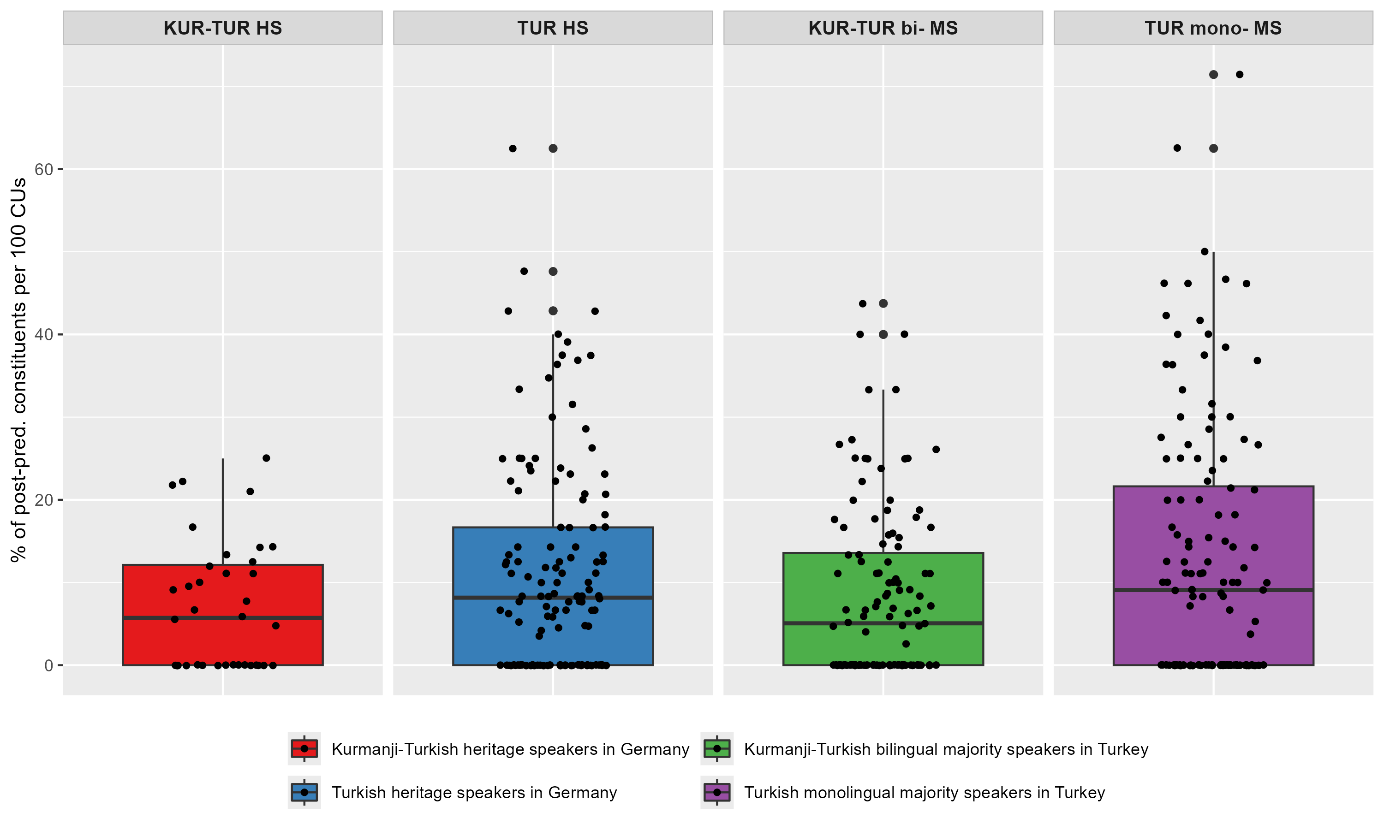
\includegraphics[width=\textwidth]{figures/iefremenko-img006.png}
\caption{\label{fig:5.1}Frequency distribution of post-predicate structures normalized per 100 communication units (CUs).}
\end{figure}

Figure~\ref{fig:5.1}\footnote{In this and subsequent figures, heritage speakers are abbreviated as HS and majority speakers as MS.} shows the frequency distribution of post-predicate structures normalized per 100 CUs across the four groups. The line inside each box shows the median, while each dot indicates the mean number of post-predicate structures per 100 CUs used by a speaker in a communicative situation, that is, there are four dots per each speaker.

Figure \ref{fig:5.1} visually illustrates that all groups use post-predicate structures, with Turkish monolinguals using them the most ($\bar{x}$ = 12.99), followed by Turkish heritage speakers (HS) in Germany ($\bar{x}$ = 11.3), Kurmanji-Turkish bilinguals in Turkey ($\bar{x}$ = 8.37), and Kurmanji-Turkish HS in Germany ($\bar{x}$ = 7.07). However, the figure also highlights high individual variation within each group: there are speakers who, in some of their productions, do not use post-predicate structures at all, and there are some speakers who employ post-predicate structures in more than 60\% of the CUs.


To further explore these observations, the analysis considers whether there is an effect of -lingualism and the societal status of Turkish on the use of the post-predicate position. A linear mixed-effects model was run to investigate this. The dependent variable in the model is the Percentage of Post-Predicate Structures. The fixed effect -Lingualism has two levels: monolinguals (Turkish monolingual speakers) and multilinguals (Turkish HS in Germany, Kurmanji-Turkish bilingual speakers in Turkey, and Kurmanji-Turkish HS in Germany). The second fixed effect, Societal Status, distinguishes between heritage and majority contexts. Participant is included as a random variable to account for individual variation among speakers.

\begin{table}
\begin{tabularx}{\textwidth}{XYY}
\lsptoprule
\textbf{Random effects:}\\
\midrule
\textbf{Groups} & \textbf{Variance} &\textbf{Standard Deviation} \\
    Participant (Intercept) & 1.03 & 1.01 \\
    Residual & 164.10 & 12.81 \\
    \midrule
% \lspbottomrule
\end{tabularx}
\begin{tabularx}{\textwidth}{l@{}rrrrr}
% \lsptoprule
\textbf{Fixed effects:}\\
\midrule
\textbf{Fixed effect} & \textbf{Estimate} & \textbf{Std. Error} & \textbf{df} & \textbf{t-value} & \textbf{\textit{p}-value} \\
(Intercept) & 15.01 & 1.94 & 100 & 7.73 & $<.0001^{***}$ \\
-Lingualism (multilingual) & -4.61 & 1.66 & 100 & -2.77 & $.006^{**}$ \\
Societal Status (majority) & -2.03 & 1.56 & 100 & -1.29 & .19 \\
\lspbottomrule
\end{tabularx}
\caption{\label{tab:key:5.1}Results of the linear mixed-effects model for percentage of post-predicate structures with multilingualism and societal status as fixed effects.}
\end{table}


Multilingualism: Multilingualism is an independent variable assigned the levels \textit{multilingual}, which includes Kurmanji-Turkish HS in Germany, Turkish HS in Germany, Kurmanji-Turkish bilinguals in Turkey, and \textit{monolingual}, which comprises Turkish monolinguals. As seen in Table \ref{tab:key:5.1}, there is a significant negative effect of multilingualism on the use of post-predicate structures (estimate: -4.61, SE=1.66, $p=.006$), meaning that multilingual speakers use fewer post-predicate structures compared to monolingual Turkish speakers.

Societal status: Societal status is an independent variable categorized into two levels: \textit{heritage}, which includes Kurmanji-Turkish heritage speakers in Germany and Turkish heritage speakers in Germany, and \textit{majority}, which consists of Kurmanji-Turkish bilinguals in Turkey and Turkish monolinguals. As shown in Table \ref{tab:key:5.1}, societal status does not significantly affect the use of post-predicate structures in Turkish.

To determine whether the negative effect of multilingualism is significant across all multilingual groups in the data, another linear mixed-effects model was conducted. In this model, the dependent variable is the Percentage of Post-Predicate Structures, while the fixed effect is Group, which consists of four levels: Kurmanji-Turkish heritage speakers in Germany (Detr), Turkish heritage speakers in Germany (Debi), Kurmanji-Turkish bilinguals in Turkey (Tubi), and Turkish monolinguals (Tumo). The Turkish monolingual group was selected as the reference level in the regression analysis because they demonstrated a significantly higher frequency of post-predicate structure usage compared to the multilingual groups. To account for individual variation in the speakers, Participant was included as the random variable. The results of this regression analysis are presented below.

\begin{table}
\begin{tabularx}{\textwidth}{XYY}
\lsptoprule
\textbf{Random effects:}\\
\midrule
\textbf{Groups} & \textbf{Variance} & \textbf{Standard} \textbf{Deviation}\\
Participant (Intercept) & 0.18 & 0.42\\
Residual & 164.10 & 12.81\\
\midrule
\end{tabularx}
\begin{tabularx}{\textwidth}{Xrrrrr}
% \lsptoprule
\textbf{Fixed effects:}\\
\midrule
\textbf{Fixed effect} & \textbf{Estimate} & \textbf{Std. Error} & \textbf{df}  & \textbf{t-value} & \textbf{\textit{p}-value}\\
Intercept & 12.98 & 1.13 & 99 & 11.44 & $<.0001^{***}$\\
Group (Debi) & -1.68 & 1.59 & 99 & -1.05 & .29\\
Group (Detr) & -5.91 & 2.42 & 99 & -2.44 & $.01^{**}$\\
Group (Tubi) & -4.61 & 1.64 & 99 & -2.80 & $.006^{**}$\\
\lspbottomrule
\end{tabularx}
\caption{\label{tab:key:5.2}Regression results for linear mixed-effects model with percentage of post-predicate structures as the dependent variable and group as the fixed effect.}
\end{table}

Group: Group is an independent variable assigned the levels \textit{Kurmanji-Turkish HS in Germany (Detr)}, \textit{Turkish HS in Germany (Debi)}, \textit{Kurmanji-Turkish bilinguals in Turkey (Tubi)}, and \textit{Turkish monolinguals (Tumo)}. The reference level is Turkish monolinguals. As seen in \tabref{tab:key:5.2}, Kurmanji-Turkish HS in Germany (Detr) and Kurmanji-Turkish bilinguals in Turkey (Tubi) tend to employ significantly fewer post-predicate structures compared to the monolinguals, but there is no significant difference between Turkish HS in Germany and Turkish monolinguals.

To summarize the findings so far, no increased frequency of the post-predicate position has been observed in multilinguals. In fact, the analysis indicates that monolinguals in Turkey are the group that employs the highest number of post-predicate structures. Furthermore, the regression analysis also revealed that while Kurmanji-Turkish HS in Germany and Kurmanji-Turkish bilinguals in Turkey tend to employ significantly fewer post-predicate structures compared to the monolinguals, there is no significant difference between Turkish HS in Germany and Turkish monolinguals. Interestingly, it is the groups with Kurmanji as the contact language that tend to use significantly fewer post-predicate structures than monolinguals. This finding may suggest the influence of Kurmanji, a predominantly SOV language, on word order in Turkish. Furthermore, the analyses indicate that societal status does not seem to influence the use of post-predicate structures, as no differences are observed between heritage and majority Turkish speakers. Finally, it is important to emphasize the considerable individual variation within these groups: some speakers do not use post-predicate structures at all in certain productions, while others employ this position in more than 60\% of their utterances.

\section[The use of post-predicate constituents in Turkish]{The use of post-predicate constituents in Turkish across communicative situations}\label{sec:key:5.2}

Thus far, observations indicate that Kurmanji-speaking groups (Kurmanji-Turkish HS in Germany and Kurmanji-Turkish bilinguals in Turkey) tend to employ post-predicate structures less frequently than non-Kurmanji-speaking groups. This suggests that Kurmanji, as an SOV language, may influence word order in Turkish, leading speakers to prefer the verb-final pattern, which is common to both languages.

However, before drawing conclusions about the influence of Kurmanji on Turkish, it is crucial to analyze the distribution of post-predicate structures across the four communicative situations, as the employment of post-predicate structures in Turkish is sensitive to formality and mode. As explained in \sectref{sec:key:3.1.1}, this position is frequently employed in informal situations, particularly in spoken mode, and there is normative pressure on its use in formal situations, especially in the written mode (\citealt{Erguvanli1984}, \citealt{Schroeder1995}). The method `Language Situations' used in this study was designed in such a way that each speaker produced narrations in four communicative situations—informal spoken, informal written, formal spoken, and formal written—that provided an opportunity to control the data for formality (formal vs. informal) and mode (spoken vs. written). The following analysis presents the frequency distribution of post-predicate structures across these four communicative situations.

\begin{figure}
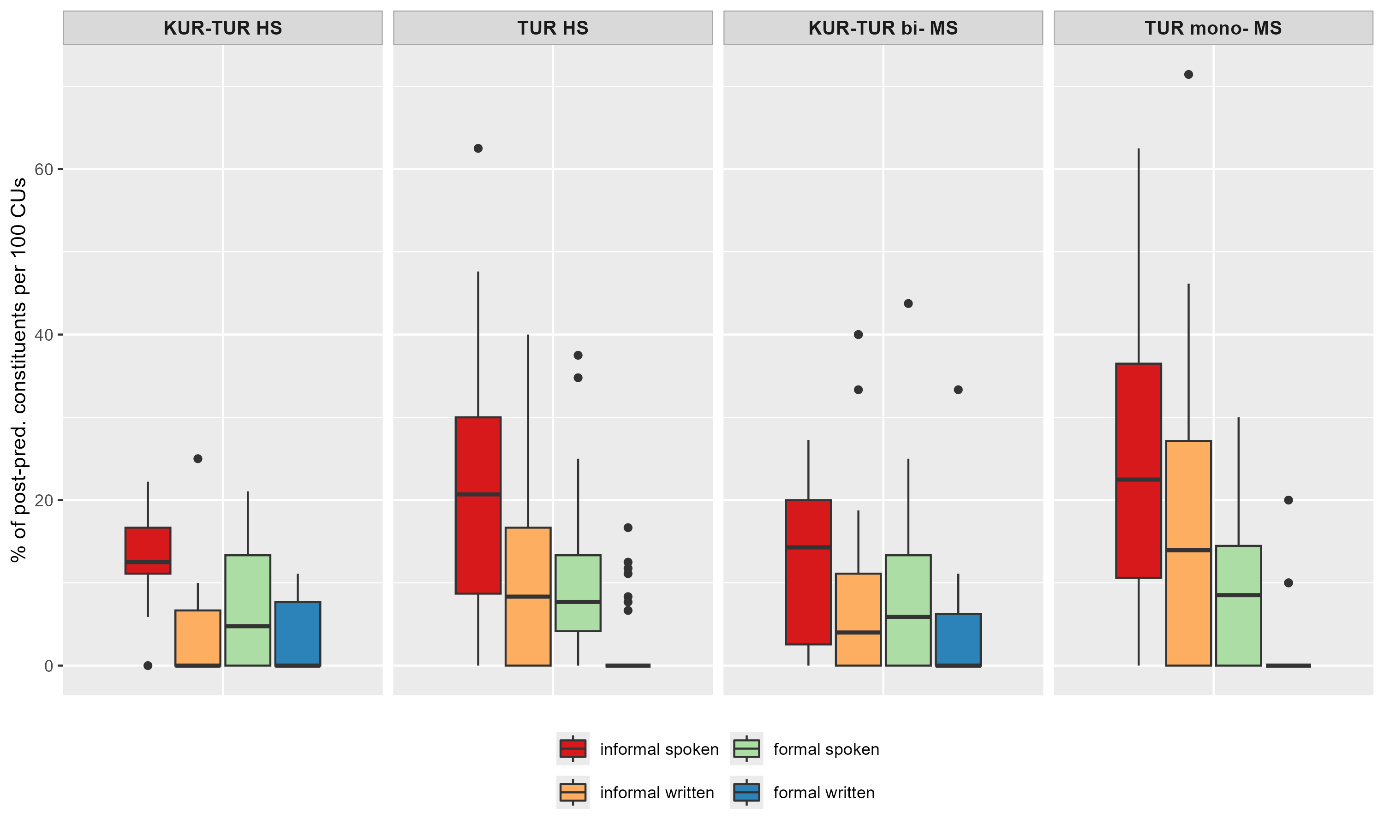
\includegraphics[width=\textwidth]{figures/iefremenko-img007.png}
\caption{Frequency distribution of post-predicate structures in Turkish, normalized to 100 CUs, with a focus on formality and mode.}
\label{fig:key:8}
\end{figure}

\figref{fig:key:8} presents the frequency distribution of post-predicate structures normalized to 100 CUs across four communicative situations. The line inside each box represents the median, while black dots, which fall outside the whiskers' range, are outliers.

\figref{fig:key:8} demonstrates a common pattern in the frequency distribution of post-predicate structures across the four groups. Across groups, the highest number of post-predicate structures occurs in the informal spoken situation: Kurmanji-Turkish HS in Germany ($\bar{x}$=12.93), Turkish HS in Germany ($\bar{x}$=21.75), Kurmanji-Turkish bilinguals in Turkey ($\bar{x}$=12.68), and Turkish monolinguals ($\bar{x}$=23.74). The informal written situation shows intermediate values: Kurmanji-Turkish HS in Germany ($\bar{x}$=5.25), Turkish HS in Germany ($\bar{x}$=10.84), Kurmanji-Turkish bilinguals in Turkey ($\bar{x}$=8.20), and Turkish monolinguals ($\bar{x}$=17.63). The formal spoken situation is also intermediate: Kurmanji-Turkish HS in Germany ($\bar{x}$=6.99), Turkish HS in Germany ($\bar{x}$=10.37), Kurmanji-Turkish bilinguals in Turkey ($\bar{x}$=9.06), and Turkish monolinguals ($\bar{x}$=9.33). The lowest number of post-predicate structures occurs in the formal written situation: Kurmanji-Turkish HS in Germany ($\bar{x}$=3.10), Turkish HS in Germany ($\bar{x}$=2.26), Kurmanji-Turkish bilinguals in Turkey ($\bar{x}$=3.54), and Turkish monolinguals ($\bar{x}$=1.25). Overall, informal written and formal spoken productions are intermediate, although in the monolingual group, the informal written mean ($\bar{x}$=17.63) is higher than the formal spoken mean ($\bar{x}$=9.33).

First of all, \figref{fig:key:8} demonstrates that there is roughly a common pattern in the frequency distribution of post-predicative structures across the four groups: the highest number of post-predicate structures is used in the informal spoken communicative situation and the lowest number of such structures is used in the formal written communicative situation. The informal written and the formal spoken productions are in the middle, with roughly a similar number of post-predicate structures. Although, in the monolingual group, the number of post-predicate structures in the informal written situation is higher than in the formal spoken one. Specifically, \textbf{\textmd{Kurmanji-Turkish HS in Germany}} produce on average $\bar{x}$={12.93} in informal spoken, $\bar{x}$={5.25} in informal written, $\bar{x}$={6.99} in formal spoken, and $\bar{x}$={3.10} in formal written. \textbf{\textmd{Turkish HS in Germany}} produce $\bar{x}$={21.75}, $\bar{x}$={10.84}, $\bar{x}$={10.37}, and $\bar{x}$={2.26}. \textbf{\textmd{Kurmanji-Turkish bilinguals in Turkey}} produce $\bar{x}$={12.68}, $\bar{x}$={8.20}, $\bar{x}$={9.06}, and $\bar{x}$={3.54}. \textbf{\textmd{Turkish monolinguals}} produce $\bar{x}$={23.74}, $\bar{x}$={17.63}, $\bar{x}$={9.33}, and $\bar{x}$={1.25} in informal spoken, informal written, formal spoken, and formal written situations, respectively.


Furthermore, \figref{fig:key:8} also shows that in terms of the frequency distribution of post-predicate structures, Turkish HS in Germany behave similarly to monolinguals, while Kurmanji-Turkish HS in Germany is similar to Kurmanji-Turkish bilinguals in Turkey, with the difference between the communicative situations being more pronounced in the first two groups. In other words, similar patterns in frequency distribution are found in the groups with Kurmanji as the contact language and in the groups without Kurmanji as the contact language.

To find out whether formality and mode modulate the employment of post-predicate structures in each of the four groups, a linear mixed-effects model was conducted. In this model, the dependent variable is the Percentage of Post-Predicate Structures, while the fixed effects include the interaction between Formality and Mode, nested within the variable Group. The variable Participant is included as a random effect to account for individual variation.\footnote{Rather than fitting a full factorial model including all possible interactions between Formality, Mode, and Group, the analysis focuses on theoretically motivated contrasts within each group. This approach allows the model to directly test whether the effects of formality and mode differ across the four speaker groups while avoiding unnecessary higher-order interactions that are not central to the hypotheses and would substantially increase model complexity.}


% ------------------------
\begin{sidewaystable}
\begin{tabularx}{\textwidth}{XYY}
\lsptoprule
\textbf{Random effects:}\\
\midrule
\textbf{Groups} & \textbf{Variance} & \textbf{Standard Deviation}\\
Participant (Intercept) & 13.06 & 3.64\\
Residual & 112.58 & 10.61\\
\midrule
\end{tabularx}
\begin{tabularx}{\textwidth}{lrrrrr}
% \lsptoprule
\textbf{Fixed effects:}\\
\midrule
% \lsptoprule
\textbf{Fixed effect} & \textbf{Estimate} & \textbf{Standard Error} & \textbf{df}  & \textbf{t-value} & \textbf{\textit{p}-value}\\
(Intercept) & 9.32 & 1.98 & 383.56 & 4.70 & < $.0001^{***}$\\
Group (Debi) & 1.04 & 2.78 & 383.56 & 0.37 & .70\\
Group (Detr) & -2.33 & 4.22 & 383.56 & -0.55 & .58\\
Group (Tubi) & -0.26 & 2.87 & 383.56 & -0.093 & .92\\
Group (Tumo)\_Formality (informal) & 14.41 & 2.65 & 297.00 & 5.43 & < $.0001^{***}$\\
Group (Debi)\_Formality (informal) & 11.38 & 2.61 & 297.00 & 4.35 & < $.0001^{***}$\\
Group (Detr)\_Formality (informal) & 5.93 & 5.00 & 297.00 & 1.18 & .23\\
Group (Tubi)\_Formality (informal) & 3.61 & 2.78 & 297.00 & 1.29 & .19\\
Group (Tumo)\_Mode (written) & -8.07 & 2.65 & 297.00 & -3.04 & $.003^{**}$\\
Group (Debi)\_Mode (written) & -8.10 & 2.61 & 297.00 & -3.10 & $.002^{**}$\\
Group (Detr)\_Mode (written) & -3.89 & 5.00 & 297.00 & -0.77 & .43\\
Group (Tubi)\_Mode (written) & -5.52 & 2.78 & 297.00 & -1.98 & $.04^{*}$\\
Group (Tumo)\_Formality (informal)\_mode (written) & 1.97 & 3.75 & 297.00 & 0.53 & 0.59\\
Group (Debi)\_Formality (informal)\_mode (written) & -2.81 & 3.69 & 297.00 & -0.76 & 0.45\\
Group (Detr)\_Formality (informal)\_mode (written) & -3.79 & 7.07 & 297.00 & -0.54 & 0.59\\
Group (Tubi)\_Formality (informal)\_mode (written) & 1.04 & 3.94 & 297.00 & 0.26 & 0.79\\
\lspbottomrule
\end{tabularx}

\caption{\label{tab:key:5.3} Regression results for linear mixed-effects model with percentage of post-predicate structures as the dependent variable and formality and mode as fixed effects.}
\end{sidewaystable}


Table \ref{tab:key:5.3} indicates that both formality and mode significantly affect the use of post-predicate structures in Turkish monolinguals and Turkish HS in Germany. Specifically, these groups tend to use more post-predicate structures in informal situations, with the highest frequencies observed in informal spoken communicative situations and lower frequencies in formal written communicative situations. In contrast, formality does not have a significant effect on post-predicate structure use in Kurmanji-Turkish HS in Germany or in Turkish bilingual speakers in Turkey, suggesting that these groups employ post-predicate structures at a more consistent rate across different communicative situations. Regarding mode, it affects the frequency of post-predicate structures in Turkish bilingual speakers in Turkey, who produce fewer post-predicate structures in the written than in the spoken communicative situations, but not in Kurmanji-Turkish HS in Germany. Overall, this suggests that while Turkish monolinguals and Turkish HS in Germany exhibit clear distinctions between communicative situations, Turkish bilingual speakers in Turkey show no significant differences in terms of formality, and Kurmanji-Turkish HS in Germany show no significant differences in either formality or mode. This pattern may be attributed to the lack of register flexibility in these groups, defined as the limited ability to adapt linguistic resources — at the lexical, syntactic, and discourse levels — according to the communicative context at hand (\citealt{QinUccelli2020}). The phenomenon of register flexibility will be further discussed in \sectref{sec:key:7.3}.

Beyond the group differences, analyzing the use of the post-predicate position across various communicative situations offers empirically grounded insights into the effect of formality and mode, discussed in the descriptive grammars of Turkish (\citealt{Erguvanli1984}, \citealt{Kornfilt1997}). As described in \sectref{sec:key:3.1.1}, the post-predicate position in an (S)OV language Turkish is typical of informal situations, while in formal situations it occurs rarely (\citealt{Erguvanli1984}, \citealt{Schroeder1995}). \citet{Erguvanli1984} notes that in more formal registers of Standard Turkish, such as legal documents and news reports -- whether in written form or broadcasted on radio and television—post-predicate structures are exceptionally uncommon. This scarcity can be attributed, in part, to normative pressures that discourage the use of post-predicate structures in formal settings.

Such claims can be partially confirmed by the data: As illustrated in \figref{fig:key:8}, a significant number of post-predicate structures are present in the formal spoken communicative situation, which is an oral witness report in the data. The example \REF{ex:key:38} below demonstrates the use of this position in the formal spoken situation by a monolingual speaker.

\ea%38
  \label{ex:key:38} Turkish, TUmo10MT\_fsT \\

        \gll Ee  karşı-dan   park-ta    yaşa-n-dı    bu  olay\\
hm  opposite-\textsc{abl}  park\textsc{-loc}  live-\textsc{pass-pst.3sg}  this  event\\
\glt ‘This incident happened hmm across the street in the park’.  \\
  \z

Interestingly, the use of post-predicate structures is frequent in the formal spoken communicative situation in the four groups, regardless of the societal status of Turkish -- whether it is the majority language or the heritage language. This indicates that even those speakers who receive education in Turkish and are exposed to its formal register employ post-predicate structures in the formal spoken situation.

On the contrary, what the data do confirm is the avoidance of the post-predicate structures in formal written texts. For instance, within the monolingual data, post-predicate structures appear in written witness reports but are exceedingly rare, with an average of just 1.25 occurrences per 100, namely four instances across 32 speakers.

The example \REF{ex:key:39} illustrates the use of the post-predicate position in the formal written situation by a monolingual Turkish speaker. In this instance, the subject of the main clause, \textit{öndeki mavi araba} (‘the blue car at the front’), appears in the post-predicate position, despite the fact that the text is a written witness report, which belongs to the formal setting.

\ea%39
  \label{ex:key:39} Turkish, TUmo32FT\_fwT \\
     \gll Köpek    yol-un    orta-sın-a    koş-unca  ani    fren\\
dog    road-\textsc{gen}  middle-\textsc{poss-dat}  run-\textsc{cvb}  sudden    brake\\
\\
\gll yap-mak  zorunda  kal-dı    \textit{ön-de-ki} \textit{mavi} \textit{araba}. \\
do\textsc{-inf}   must    stay-\textsc{pst.3sg}  front\textsc{-loc-attr}  blue  car\\
\glt ‘When the dog ran into the middle of the road, the blue car at the front had to brake immediately.’ 
  \z

The tendency to avoid post-predicate structures in the formal written situation is maintained also in the heritage groups in Germany. As illustrated in \figref{fig:key:8}, the use of post-predicate constituents in formal written situations is significantly lower than in the other situations, with an average of 2.26 instances per 100 CUs in Turkish HS in Germany and 3.1 in Kurmanji-Turkish HS in Germany. This finding is somewhat surprising, considering that heritage speakers receive little to no formal education in their heritage language and are generally not exposed to formal registers.

At the same time, the group that uses the highest number of post-predicate structures in the formal written situation is Kurmanji-Turkish bilinguals in Turkey. This finding is also surprising because, unlike heritage speakers in Germany, for bilinguals in Turkey, Turkish is the majority language, and they get formal education in it, similar to the monolinguals. However, the absolute number of such examples is too small to draw any definitive conclusions, with 10 instances across 30 speakers.

To sum up, the analysis of post-predicate structures across the four communicative situations revealed a consistent pattern across all groups: post-predicate structures are used most frequently in the informal spoken situation, followed by informal written and formal spoken situations, with their lowest occurrence in the formal written communicative situation. It is important to note that this pattern is most pronounced among Turkish monolinguals and Turkish HS in Germany. The regression model further showed that in Turkish monolinguals and Turkish HS in Germany, the use of the post-predicate position is strongly influenced by formality and mode. In contrast, Turkish bilinguals in Turkey and Kurmanji-Turkish HS in Germany show no significant difference between the formal and the informal communicative situations. Additionally, mode has no effect on post-predicate usage in Kurmanji-Turkish HS in Germany.

These findings suggest that Turkish bilinguals in Turkey and Kurmanji-Turkish HS in Germany do not distinguish between communicative situations to the same extent as Turkish monolinguals and Turkish HS in Germany. This points to the register inflexibility among speakers of Kurmanji, a phenomenon that will be discussed further in \sectref{sec:key:7.3}.

\section{Composition of post-predicate constituents}\label{sec:key:5.3}

So far, the frequency analysis showed a lower frequency of post-predicate structures in multilinguals compared to monolinguals. However, the difference is significant only in the groups that have Kurmanji in their repertoire, and these differences appear to result from blurred distinctions between formal and informal language, or between spoken and written language, in these groups.

While these findings reveal an overall trend, they do not yet clarify whether the composition of post-predicate structures differs across the groups. To address this, post-predicate structures will be analyzed with a focus on their weight, types, and semantic roles. This investigation will provide deeper insight into the linguistic developments at play and help explain why post-predicate structures are less frequent in groups with Kurmanji as a contact language compared to those without.

\subsection{Weight of post-predicate constituents in Turkish}\label{sec:key:5.3.1}

The quantitative analysis, described in \sectref{sec:key:5.1}, showed the frequency distribution of post-predicate structures in general, without considering the number of constituents that occur post-predicatively. The analysis of weight will show whether there are differences in the length of structures in the post-predicate position across the groups.

Following \citet{HaigEtAl2024}, four weight types of post-predicative constituents are distinguished: weight 1 consists of a single phonological word, weight 2 includes two phonological words, weight 3 includes three phonological words, and weight 4 comprises four or more phonological words.  Below is an example from the data for each weight type, with the post-predicate constituents in italic.\\

\begin{itemize}
\item{Weight 1:} a single phonological word.
\ea%40
  \label{ex:key:40} Turkish, TUbi14FT\_isT \\
     \gll Çocuk  araba-sı  var-dı    \textit{el-in-de}. \\
child  car-\textsc{poss}  be-\textsc{pst.3sg}  hand-\textsc{poss-loc}\\
\glt ‘A stroller was in her hands.’ 
  \z

\item{Weight 2:} two phonological words.

\ea%41
  \label{ex:key:41} Turkish, DEtr02FT\_fsT \\
     \gll Az   önce   bi   kadın-ı    gör-dü-m  \textit{eş-i-ylen}.   \textit{beraber}\\
little  before  \textsc{art}  woman-\textsc{acc}  see\textsc{-pst-1sg}  spouse-\textsc{poss-inst}  together \\
\glt ‘Just now I saw a woman together with her husband.’ 
  \z

\item{Weight 3:} three phonological words.

\ea%42
  \label{ex:key:42}  Turkish, TUmo32FT\_fsT \\
     \gll Yeni  bi  apartman  yap-ıl-dı   \\
new  \textsc{art}  block    do-\textsc{pass-pst.3sg}\\

        \gll \textit{onun}  \textit{orda-ki}    \textit{köşe-sin-de}.\\
his  there-\textsc{attr}  corner-\textsc{poss-loc}.\\
\glt ‘A new apartment building was built at that corner.’
  \z

\item{Weight 4:} four or more phonological words.

\ea%43
  \label{ex:key:43} Turkish, TUmo24MT\_isT \\
     \gll Ee  on-dan  sonra  firen-e    bas-tı    \textit{o}  \textit{gel-en} \textit{iki} \\
            hm  after  that  brake-\textsc{dat}  press\textsc{-pst.3sg}  that  come-\textsc{part}  two  \\
    \gll \textit{araba-dan}  \textit{ön-de-ki}.\\
                    car-\textsc{abl}  front\textsc{-loc-attr}  \\
\glt ‘Hm, and then braked, the front car out of those two that were coming.’ 
  \z
\end{itemize}

Elements are counted as separate words if they contribute independently to the phonological or semantic weight of a constituent, such as postpositions, discourse markers, connectors, and doubled expressions (\emph{yavaş yavaş} ‘slowly,’ \emph{sık sık} ‘often’) or the indefinite article \emph{bir} ‘a/an.’ Clitics like \textit{-y(lA)}/\textit{{}-ile} ‘with’ or \textit{-y(sA)}/\textit{{}-ise} ‘if’ are excluded because they attach phonologically to a host word and do not add independent prosodic or lexical weight.

The analysis of the weight of post-predicate constituents across the four speaker groups is presented below.

\begin{figure}
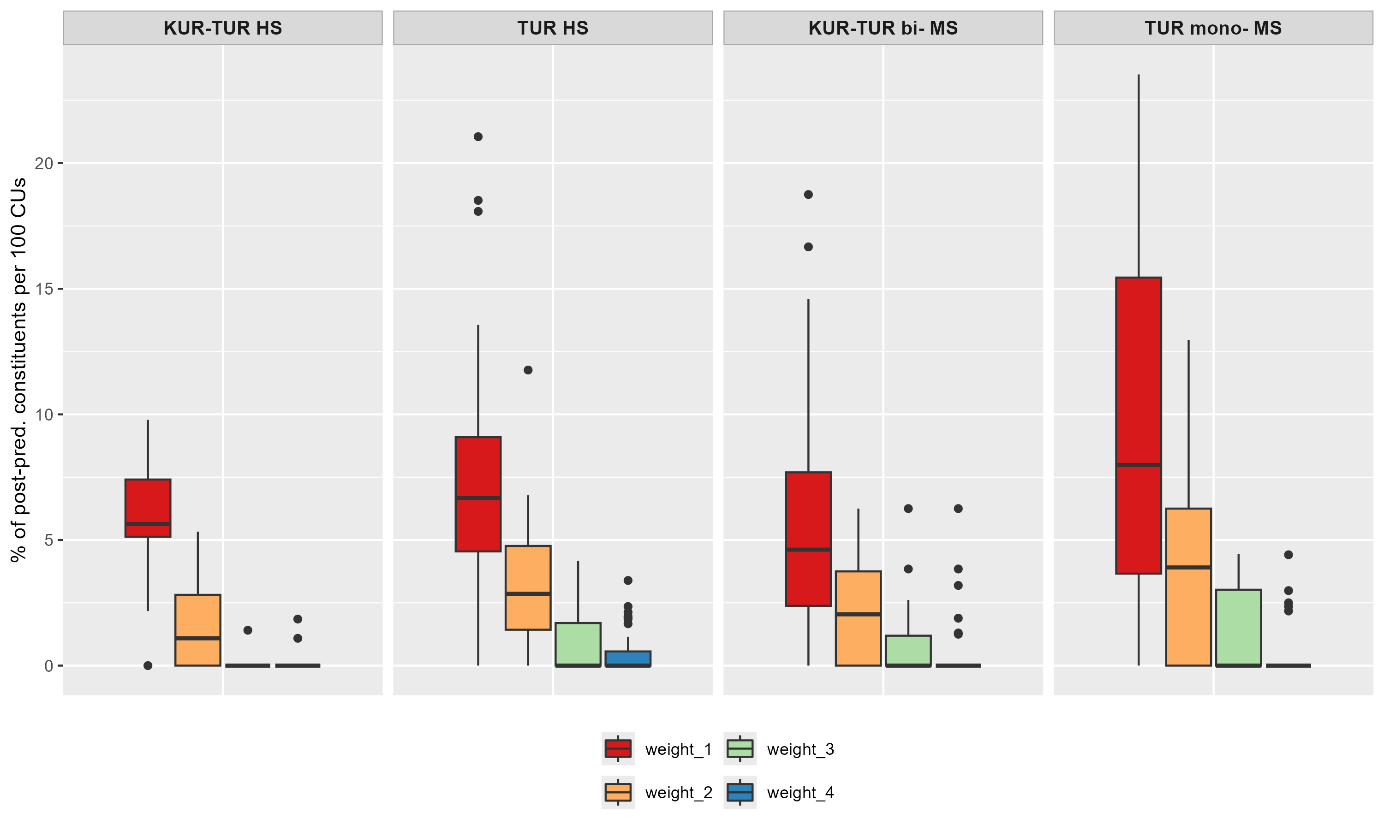
\includegraphics[width=\textwidth]{figures/iefremenko-img008.png}
\caption{Frequency distribution of post-predicate structures with a different weight.}
\label{fig:key:9}
\end{figure}

\figref{fig:key:9} shows the frequency distribution of post-predicate structures with a different weight. The line inside each box represents the median, while black dots, which fall outside the whiskers' range, are outliers. The percentage of post-predicate structures with a particular weight was calculated in relation to 100 CUs. \figref{fig:key:9} also indicates that in terms of the weight of post-predicate constituents, speakers of the four groups behave similarly. All speaker groups predominantly place one or two phonological words in the post-predicate position, and less frequently three, four, or more phonological words. Specifically, \textbf{\textmd{Kurmanji-Turkish HS in Germany}} produce on average $\bar{x}$={5.55} for weight 1, $\bar{x}${=1.75} for weight 2, $\bar{x}$={0.16} for weight 3, and $\bar{x}$={0.33} for weight 4 per 100 CUs. \textbf{\textmd{Turkish HS in Germany}} produce $\bar{x}${= 7.46, 3.06, 0.76,} and {0.51,} respectively. \textbf{\textmd{Kurmanji-Turkish bilinguals in Turkey}} produce $\bar{x}${=6.06 2.22, 0.71,} and {0.61}, while \textbf{\textmd{Turkish monolinguals}} produce $\bar{x}${=9.06, 4.00, 1.26,} {0.45} for weights 1 through 4, respectively. The whiskers also indicate significant individual variation within each group, particularly among the monolingual speakers in Turkey.

To determine whether there are differences between the groups regarding the weight of post-predicate constituents, a linear mixed-effects model was conducted, with the Percentage of Post-Predicate Structures with Different Weights as the dependent variable and Weight nested within the variable Group as the fixed effects. Treatment coding was applied to the Weight variable, while sum coding was used for the Group variable. The results of the regression analysis are presented in \tabref{tab:key:5.4}.

\begin{table}\small
\begin{tabularx}{\textwidth}{XYY}
\lsptoprule
\textbf{Random effects:}\\
\midrule
\textbf{Groups} & \textbf{Variance} & \textbf{Standard Deviation}\\
Participant (Intercept) & 1.03 & 1.01\\
Residual & 9.84 & 3.13\\
\midrule
\end{tabularx}
\begin{tabularx}{\textwidth}{Xrrrrr}
% \lsptoprule
\textbf{Fixed effects:}\\
\midrule
\textbf{Fixed effect} & \textbf{Estimate} & \textbf{Std. Error} & \textbf{df} & \textbf{t-value} & \textbf{\textit{p}-value}\\
(Intercept) & 7.03 & 0.37 & 385.59 & 18.73 & $<.0001^{***}$\\
Group (Debi) & 0.42 & 0.55 & 385.59 & 0.77 & .44\\
Group (Detr) & -1.48 & 0.86 & 385.59 & -1.72 & .08\\
Group (Tubi) & -0.97 & 0.57 & 385.59 & -1.69 & .09\\
groupDebi:Weight\_2 & -4.39 & 0.77 & 297.00 & -5.68 & $<.0001^{***}$\\
GroupDetr:Weight\_2 & -3.79 & 1.47 & 297.00 & -2.56 & $.01^{*}$\\
groupTubi:Weight\_2 & -3.84 & 0.82 & 297.00 & -4.66 & $<.0001^{***}$\\
GroupTumo:Weight\_2 & -5.06 & 0.78 & 297.00 & -6.45 & $<.0001^{***}$\\
GroupDebi:Weight\_3 & -6.70 & 0.77 & 297.00 & -8.67 & $<.0001^{***}$\\
GroupDetr:Weight\_3 & -5.39 & 1.47 & 297.00 & -3.64 & $.0003^{***}$\\
GroupTubi:Weight\_3 & -5.35 & 0.82 & 297.00 & -6.49 & $<.0001^{***}$\\
GroupTumo:Weight\_3 & -7.80 & 0.78 & 297.00 & -9.95 & $<.0001^{***}$\\
GroupDebi:Weight\_4 & -6.94 & 0.77 & 297.00 & -8.98 & $<.0001^{***}$\\
GroupDetr:Weight\_4 & -5.22 & 1.47 & 297.00 & -3.52 & $.0004^{***}$\\
GroupTubi:Weight\_4 & -5.44 & 0.82 & 297.00 & -6.61 & $<.0001^{***}$\\
GroupTumo:Weight\_4 & -8.61 & 0.78 & 297.00 & -10.98 & $<.0001^{***}$\\
\lspbottomrule
\end{tabularx}
\caption{\label{tab:key:5.4}Regression table for lmer with the dependent variable Percentage of Post-Predicate Structures with different weights and the fixed effects weight nested with Group.}
\end{table}

Group: Group is an independent variable assigned the levels \textit{Kurmanji-Turkish HS in Germany (Detr)}, \textit{Turkish HS in Germany (Debi)},\textit{Kurmanji-Turkish bilinguals in Turkey (Tubi)}, and \textit{Turkish monolinguals (Tumo)}. Sum coding was used for this variable.

Weight: Weight is an independent variable assigned the levels \textit{weight\_1}, \textit{weight\_2}, \textit{weight\_3}, and \textit{weight\_4}. The model showed that speakers of the four groups use one-word post-predicate constituents significantly more frequently than two-, three-, or four-word post-predicate constituents.

In summary, the analysis of weight revealed that post-predicate structures among the four speaker groups are generally short, typically consisting of one to two words. No differences in the weight of post-predicate constituents were observed between the groups, as the model indicated that one-word post-predicate constituents were used significantly more frequently than two-, three-, or four-word constituents across all four groups


\subsection{Types of post-predicate structures}\label{sec:key:5.3.2}

Next, the analysis turns to the types of post-predicate constituents. As outlined in \sectref{sec:key:3.1}, the post-predicate position is either canonical or the only possible placement for certain elements, including discourse markers, connectors, and particles. Consequently, it is crucial to investigate the types of post-predicate structures to assess whether the frequent use of one-word post-predicate constituents is influenced by the frequent employment of connectors and discourse markers in this position.

Furthermore, analyzing the types of post-predicate structures can provide insights into potential changes in the post-predicate domain of Turkish due to contact with other languages. As described in \sectref{sec:key:3.5}, German follows an (S)OV word order, but certain nominal constituents—such as prepositional phrases, determiner phrases, and adverbials—can be extraposed. In contrast, Kurmanji permits certain nominal constituents in the post-predicate position, including goals of motion, addressees of verbs of speech, and recipients of verbs of transfer. Therefore, if crosslinguistic influence is at play, a higher number of nominal constituents would be expected in groups where German and/or Kurmanji serves as the contact language.

Regarding the types of post-predicate structures, \citet{SchroederEtAl2024} distinguish five types of post-predicate elements in Turkish: nominal constituents (type 1), modal and manner adverbs (type 2), discourse markers, clitics, and connectors (type 3), non-finite clausal constituents (type 4), and finite clausal constituents (type 5). Additionally, post-predicate elements of each type can function as afterthoughts or self-repairs. As previously emphasized, this study focuses solely on non-clausal constituents in the post-predicate position, excluding afterthoughts and self-repairs from the analysis. Thus, the analysis of post-predicate constituents concentrates only on types 1-3. It is important to note that a single post-predicate structure may encompass two or more types (see example \ref{ex:key:44}), in such cases, each type is calculated separately.

\ea%44
  \label{ex:key:44} Turkish, TUbi03FT\_fsT \\
    \gll Ve (-)  kadın-ın  köpeğ-in-den  ötürü  ol-du   \\
and  {} woman-\textsc{gen}  dog-\textsc{poss-abl}  due\_to happen\textsc{-pst.3sg}   \\
    \gll  aslında    bu  kaza\\
    actually  this  accident  \\
\glt ‘Actually, this accident happened due to the woman’s dog.’  \\
    \z

For example, in example \ref{ex:key:44}, the adverb \textit{aslında} ‘actually’ and the noun phrase with the demonstrative \textit{bu kaza} ‘this accident’ are present, indicating that this example includes post-predicate structures of both type 1 and type 2.

\begin{figure} 
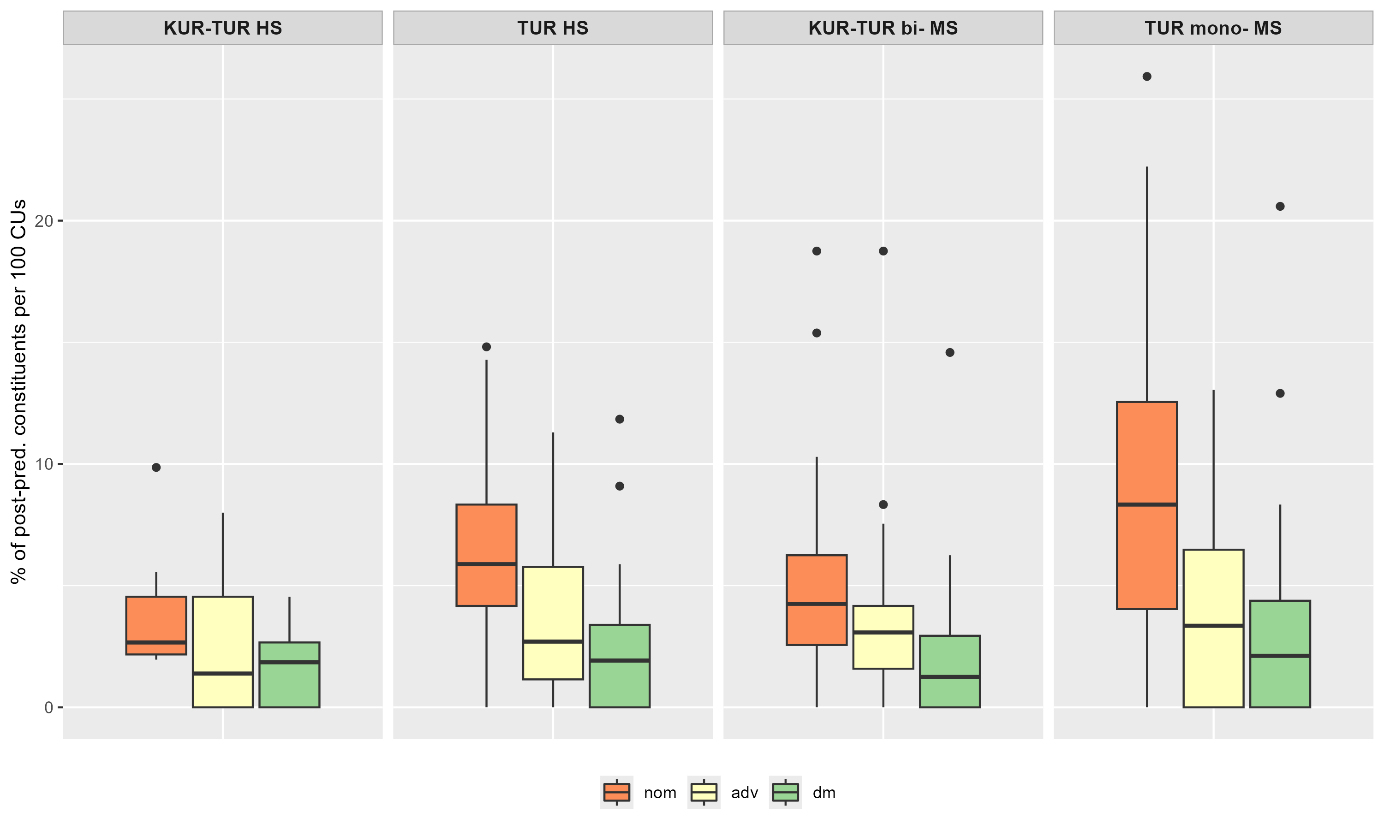
\includegraphics[width=\textwidth]{figures/iefremenko-img009.png}
\caption{\label{fig:key:10}Frequency distribution of post-predicate structures of Type 1-3 per 100 CUs. In \ref{fig:key:9}, ‘nom’ stands for nominal constituents, ‘adv’ means adverbs, while discourse markers and connectors are abbreviated as ‘dm’.}
\end{figure}
 

\figref{fig:key:10} illustrates the frequency distribution of the three types of post-predicate structures across the four groups: nominal constituents (abbreviated as \textit{nom} in the figure), modal and manner adverbs (abbreviated as \textit{adv} in the figure), and discourse markers, clitics, and connectors (abbreviated as \textit{dm} in the figure). The line within each box represents the median, while the black dots outside the whiskers indicate outliers. The percentage of post-predicate structures of each type was calculated in relation to 100 CUs.

\figref{fig:key:10} shows that the distribution of different types of post-predicate structures is relatively similar across the four groups. Nominal constituents are the most frequent type, followed by adverbs, while discourse markers and connectors occur the least frequently.

\largerpage
In terms of group differences, there are no striking disparities in the frequency distribution of adverbs, discourse markers, and connectors, although some tendencies can be observed. For nominal constituents, Turkish monolinguals exhibit the highest usage ($\bar{x}$ = 8.74), followed by Turkish heritage speakers in Germany ($\bar{x}$ = 6.78), bilingual Turkish speakers in Turkey ($\bar{x}$ = 5.10), and Kurmanji-Turkish heritage speakers in Germany ($\bar{x}$ = 3.96). For adverbs, the means are more similar across groups: Turkish monolinguals ($\bar{x}$ = 3.97), Turkish heritage speakers in Germany ($\bar{x}$ = 3.56), bilingual Turkish speakers in Turkey ($\bar{x}$ = 3.47), and Kurmanji-Turkish heritage speakers in Germany ($\bar{x}$ = 2.36). Discourse markers and connectors are the least frequent type, but still used across all groups, with the following means: Turkish monolinguals ($\bar{x}$ = 3.29), Turkish heritage speakers in Germany ($\bar{x}$ = 2.23), bilingual Turkish speakers in Turkey ($\bar{x}$ = 1.96), and Kurmanji-Turkish heritage speakers in Germany ($\bar{x}$ = 1.93). Overall, this pattern indicates that groups with Kurmanji as a contact language tend to use fewer nominal constituents in the post-predicate position compared to those without Kurmanji in their repertoire, while the distribution of adverbs and discourse markers shows less group differentiation.

To statistically verify this, a linear mixed-effects regression model was conducted with the Percentage of Post-Predicate Structures of Different Types as the dependent variable and the Type of Post-Predicate Position, nested within the variable Group, as fixed effects. Participant was included as a random variable to account for individual variation. Treatment coding was applied to the Type variable, while sum coding was used for the Group variable. The results of the regression analysis are presented in \tabref{tab:key:8}.

\begin{table}
\begin{tabularx}{\textwidth}{XYY}
\lsptoprule
\textbf{Random effects:}\\
\midrule
\textbf{Groups} & \textbf{Variance} & \textbf{Standard Deviation}\\
Participant (Intercept) & 4.20 & 2.05\\
Residual & 11.67 & 3.41\\
\midrule
% \lspbottomrule
\end{tabularx}
\begin{tabularx}{\textwidth}{Xrrrrr}
% \lsptoprule
\textbf{Fixed effects:}\\
\midrule
% \lsptoprule
\textbf{Fixed effect}  & \textbf{Estimate} & \textbf{Std. Error} & \textbf{df} & \textbf{t-value} & \textbf{\textit{p}-value}\\
(Intercept) & 3.34 & 0.45 & 260.47 & 7.36 & $<.0001^{***}$\\
Group (Debi) & 0.21 & 0.66 & 260.47 & 0.32 & .74\\
Group (Detr) & -0.98 & 1.04 & 260.47 & -0.94 & .34\\
Group (Tubi) & 0.13 & 0.69 & 260.47 & 0.15 & .85\\
GroupDebi:dm & -1.33 & 0.84 & 198.00 & -1.58 & .11\\
GroupDetr:dm & -0.42 & 1.61 & 198.00 & -0.26 & .79\\
GroupTubi:dm & -1.50 & 0.89 & 198.00 & -1.68 & .09\\
GroupTumo:dm & -0.68 & 0.85 & 198.00 & -0.80 & .42\\
GroupDebi:nom & 3.22 & 0.84 & 198.00 & 3.83 & $.0001^{***}$\\
GroupDetr:nom & 1.60 & 1.61 & 198.00 & 0.99 & .32\\
GroupTubi:nom & 1.62 & 0.89 & 198.00 & 1.81 & .07\\
GroupTumo:nom & 4.76 & 0.85 & 198.00 & 5.58 & < $.0001^{***}$\\
\lspbottomrule
\end{tabularx}
\caption{Regression table for lmer with the dependent variable Percentage of Post-Predicate Structures and the fixed effects Type nested within Group.}
\label{tab:key:8}
\end{table}

Group: Group is an independent variable assigned the levels \textit{Kurmanji-Turkish HS in Germany (Detr)}, \textit{Turkish HS in Germany (Debi)}, \textit{Kurmanji-Turkish bilinguals in Turkey (Tubi)}, and \textit{Turkish monolinguals (Tumo)}. Sum coding was used for this variable.

Type: Type is an independent variable categorized into three levels: \textit{nom} (nominal constituents), \textit{adv} (modal and manner adverbs), and \textit{dm} (discourse markers, clitics, and connectors). Treatment coding was employed, designating ‘adv’ as the reference level. The model revealed that heritage speakers of Turkish in Germany (Debi) and Turkish monolingual speakers in Turkey (Tumo) use significantly more nominal constituents. In contrast, no significant differences were observed across types for Turkish bilingual speakers in Turkey (Tubi) and Kurmanji-Turkish heritage speakers in Germany (Detr).

The regression analysis corroborated the trend illustrated in \figref{fig:key:10}, highlighting that the difference in the use of post-predicate nominal constituents is primarily between groups with and without Kurmanji as a contact language. Interestingly, the groups with no Kurmanji in their repertoire tend to use more nominal post-predicate structures compared to those with Kurmanji in their repertoire.

One of the assumptions was that a frequent use of one-word post-predicate structures among speakers in the four groups could be attributed to their frequent use of discourse markers, connectors, and particles in the post-predicate position. However, the analysis of the types of post-predicate constituents did not support this tendency across the groups. Another expectation was to find a greater number of nominal constituents in the post-predicate position among the groups with German and/or Kurmanji as a contact language compared to the monolingual group, assuming there is convergence in the post-predicate domain. Contrary to this expectation, the results revealed an opposite trend: Turkish monolinguals used the highest number of nominal constituents, while groups with Kurmanji in their repertoire employed significantly fewer nominal post-predicate structures than those without Kurmanji.

\subsection{Semantic roles of post-predicate constituents}\label{sec:key:5.3.3}
\largerpage

As described in \sectref{sec:key:3.3}, Kurmanji systematically places goals of motion, recipients of transfer, and addressees of verbs of speech in the post-predicate position. Consequently, the frequent placement of these semantic roles by Kurmanji speakers in their Turkish may indicate crosslinguistic influence in the post-predicate domain. Moreover, previous research (\citealt{Haig2020, Haignforth}) has shown that in historically SOV languages such as Turkish, goals of motion (and caused motion) are the least stable constituents. This means they are the first candidates to move into the post-predicate position in language contact situations.

In analyzing these roles, \citet{HaigEtAl2024} distinguish between various types of semantic roles. Below are examples of the most frequent ones observed in the data:

\begin{itemize}

\item Addressee of verbs of speech.

\ea%45
  \label{ex:key:45} Turkish, TUmo10MT\_isT \\
     \gll On-u  anlat-acak-tı-m  \textit{san-a} \\
it-\textsc{acc}  explain\textsc{-fut-irr-1sg}  you-\textsc{dat}\\
\glt ‘I was going to explain this to you.’
  \z

\item Benefactive -- a person who benefits or is disadvantaged by an event.

\ea%46
  \label{ex:key:46} Turkish, TUbi18MT\_isT \\
     \gll Or-da    yardım    et-ti    \textit{on-a} \\
there\textsc{-loc}  help    do-\textsc{pst.3sg}  3sg-\textsc{dat}\\
\glt‘He helped her there.’
  \z
\newpage
\item Cause -- a person/thing that is the reason for the activity.

\ea%47
  \label{ex:key:47} Turkish, TUbi06MT\_iwT \\
     \gll Az  önce  bi  köpek  ez-il-iyor-du   \textit{top} \textit{yüzünden} \\
little  before  \textsc{art}  dog  crush-\textsc{pass-prog-pst.3sg}  ball  due\_to \\
\glt ‘Just now a dog almost got run over because of a ball.’
  \z


\item Comitative -- person/thing that accompanies another person/thing in an action.


\ea%48
  \label{ex:key:48} Turkish, DEtr02FT\_fsT \\
     \gll Az   önce  bi  kadın-ı    gör-dü-m  \textit{eşi-ylen}    \textit{beraber} \\
little  before  \textsc{art}  woman-\textsc{acc}  see-\textsc{pst-1sg}  husband-\textsc{inst}    together\\
\glt ‘Just now I saw a woman together with her husband.’
  \z

\item Goals of motion and caused motion.

\ea%49
  \label{ex:key:49} Turkish, DEtr07FT\_iwT \\
     \gll Ve  {o  esnada}  köpek  top-un    arka-sın-dan    koş-tu \\
and meanwhile  dog  ball-\textsc{gen}  back-\textsc{poss-abl}  run-\textsc{pst.3sg}\\
\gll \textit{araba-nın}  \textit{peşine…}\\
 car-\textsc{gen}  after\\
\glt ‘And meanwhile, the dog ran after the ball, after the car...’
  \z

\item Static location.

\ea%50
  \label{ex:key:50} Turkish, TUmo25MT\_fsT \\
    \gll Köpek  var-dı    \textit{karşı}    \textit{taraf-ta}. \\
    dog  be-\textsc{pst.3SG}  opposite  side-\textsc{loc}  \\
    \glt ‘There was a dog on the opposite side.’
    \z

\item Source of motion.

\ea%51
  \label{ex:key:51} Turkish, DEbi18MT\_isT \\
     \gll Şöfer-ler  in-di      \textit{araba-dan} \\
driver-\textsc{pl}  {get out-\textsc{pst.3SG}} car-\textsc{abl}\\
\glt ‘The drivers got out of the car.’
  \z

\item Other -- all other categories not mentioned above. I included different semantic roles that occur very rarely in the data. It is important to mention that instances of recipients of verbs of transfer are also included in the category ‘other’ because there are only two examples of this type in the data. The reason for this lies in the methodology of the study: the video shown to the participants did not trigger the use of verbs of transfer.
\end{itemize}

\begin{figure}
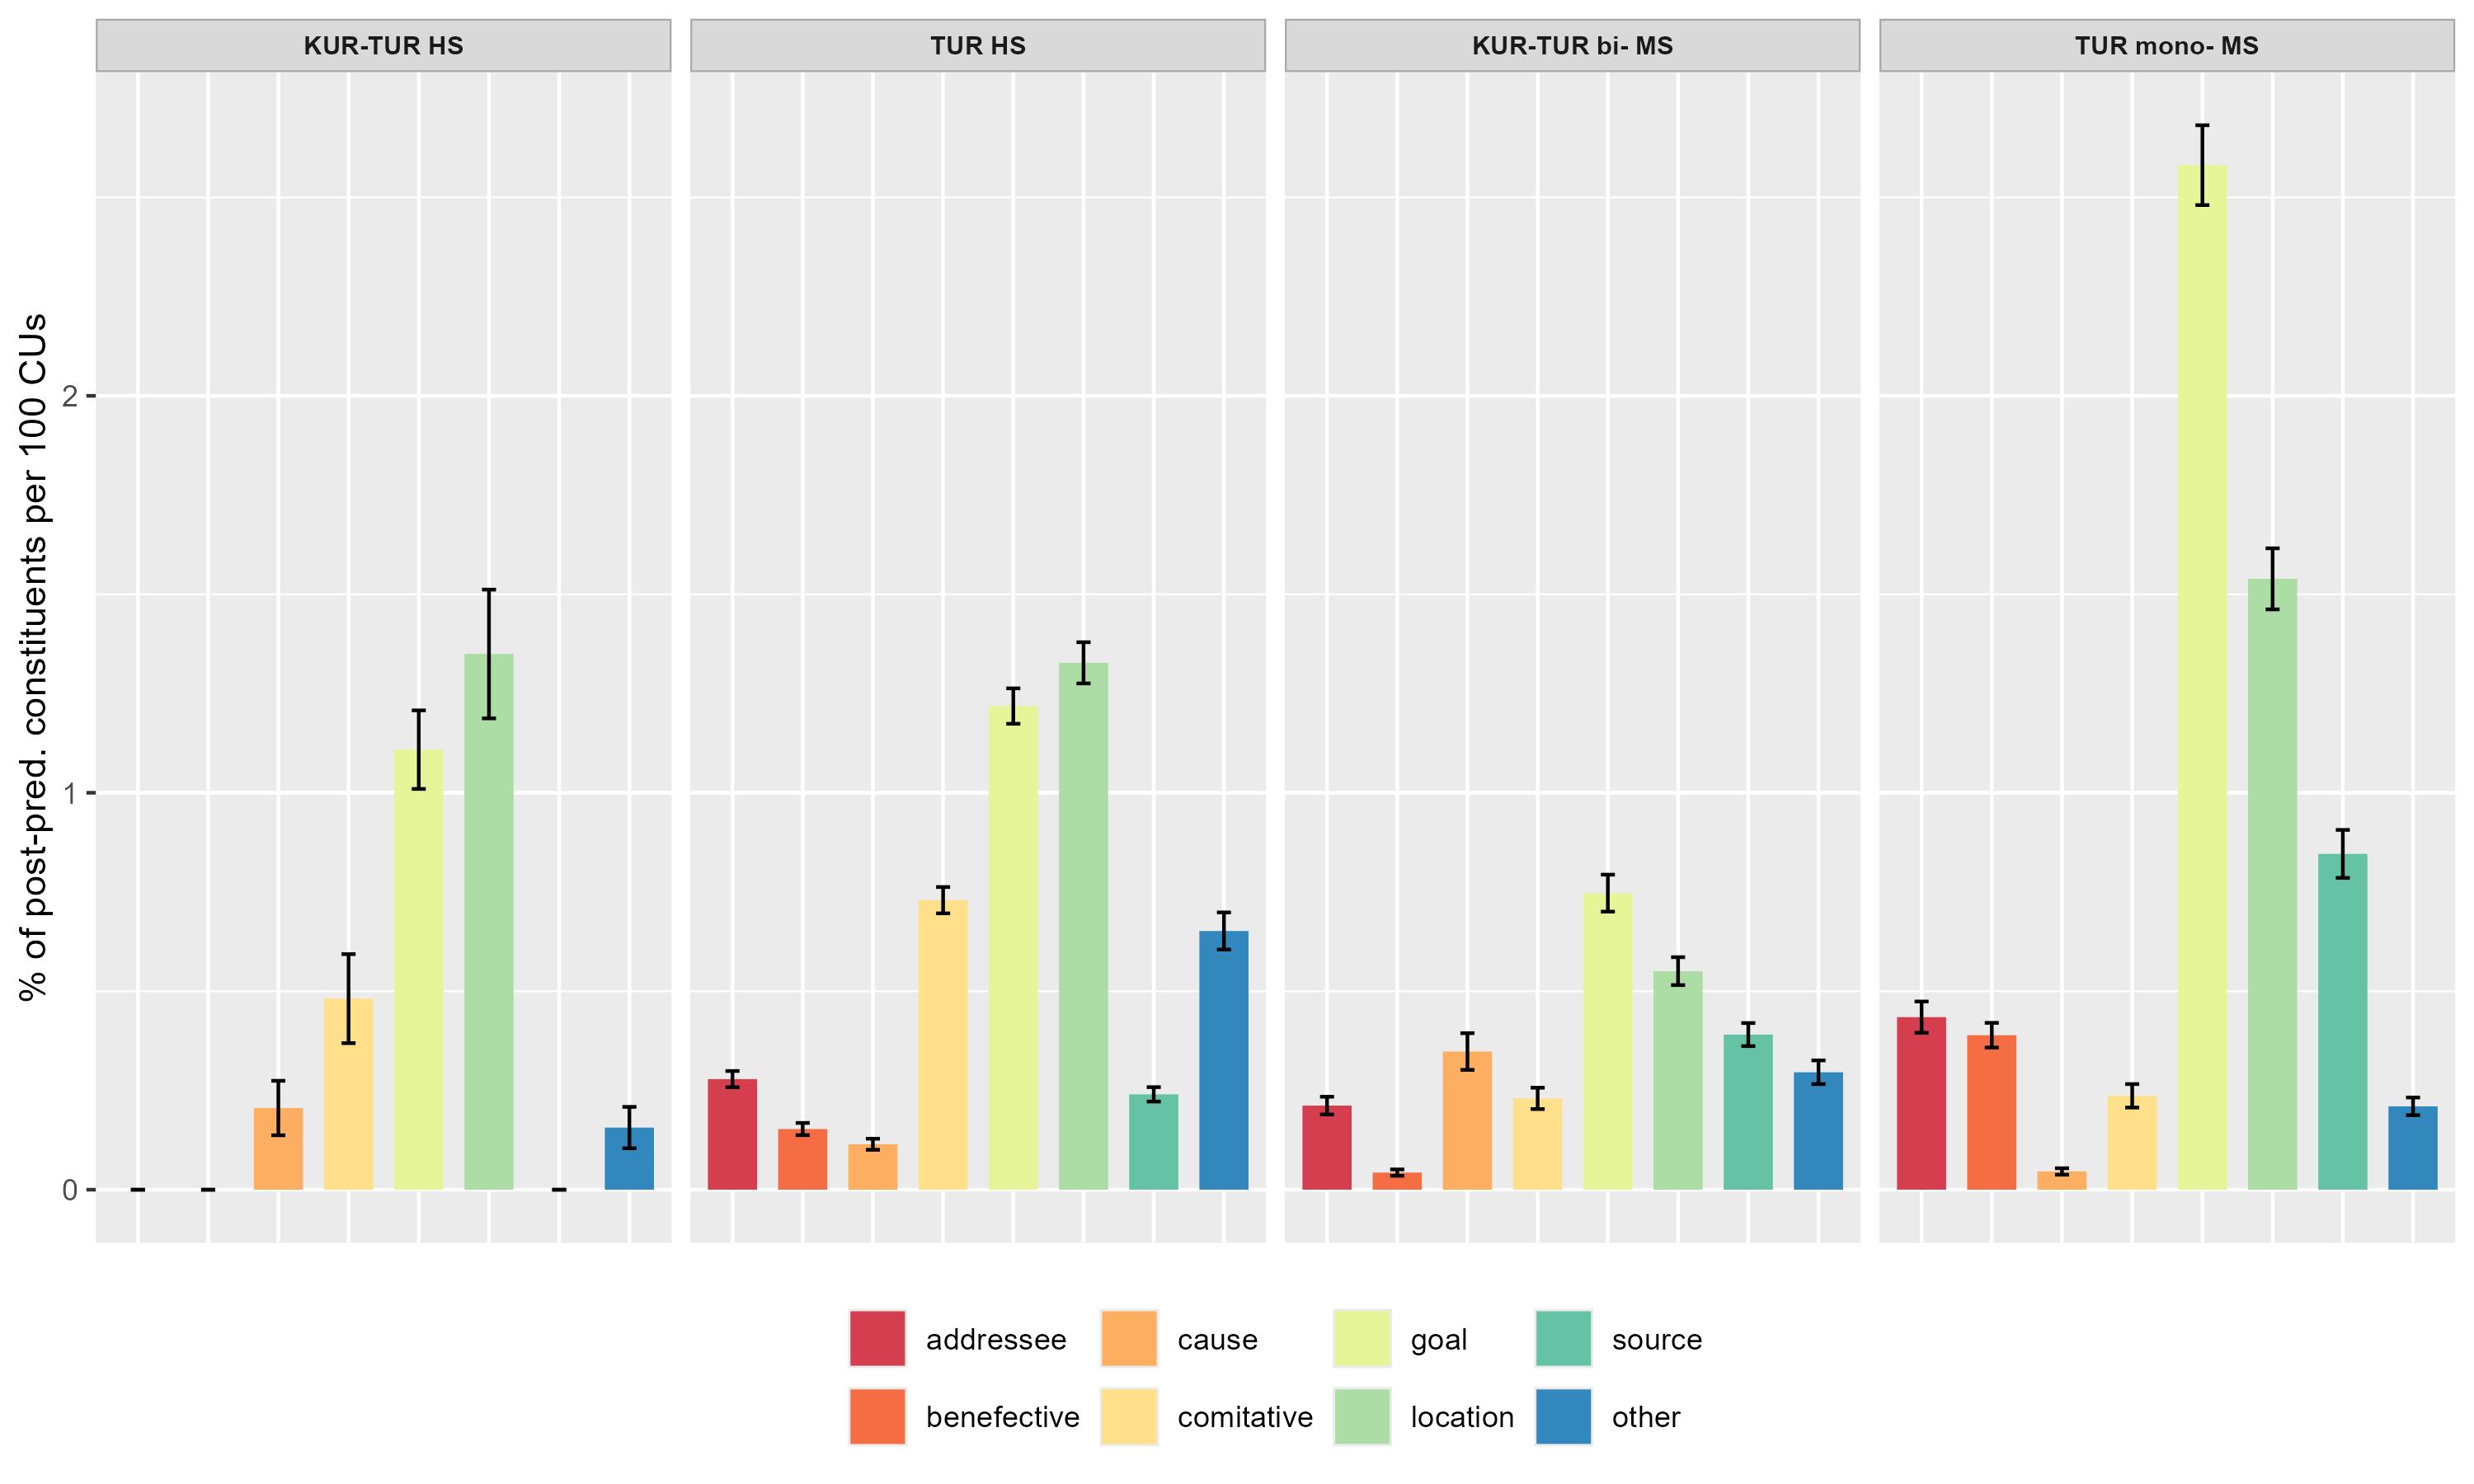
\includegraphics[width=\textwidth]{figures/iefremenko-img010.png}
\caption{\label{fig:11}Frequency distribution of nominal post-predicate structures according to their semantic role.}
\end{figure}

Figure \ref{fig:11} illustrates the mean number of nominal post-predicate structures associated with specific semantic roles, normalized by 100 CUs. Error bars indicate the standard error, providing a clearer representation of the precision of the mean estimates, particularly given the relatively low absolute numbers of nominal constituents.

According to Figure \ref{fig:11}, the most frequently occurring elements in the post-predicate position across the four groups are goals and locations. If CLI in the post-predicate domain were at play, speakers with Kurmanji in their repertoire would be expected to place motion goals, speech addressees, and recipients of transfer verbs more frequently in the post-predicate position than those without Kurmanji as a contact language. However, Figure \ref{fig:11} reveals that speakers from all groups frequently place goals of motion and caused motion in the post-predicate position, with Turkish monolingual speakers exhibiting the highest frequency of goals.

Regarding the placement of addressees of verbs of transfer in the post-predicate position, the overall numbers are quite low. Nonetheless, Figure \ref{fig:11} indicates that all groups, except for the trilinguals in Germany, do place addressees in the post-predicate position, with the monolingual group demonstrating a slightly higher percentage than the all other groups.  Given that this analysis focuses solely on nominal constituents in the post-predicate position across eight different semantic roles, there is insufficient data to run any statistical models due to the small absolute number of nominal constituents.

\subsection{Interim summary}\label{sec:key:5.3.4}

In summary, the results from the general frequency analysis of post-predicate structures, along with analyses focusing on weight, type, and semantic roles of post-predicate constituents, indicate no direct signs of CLI in the post-predicate domain. The findings reveal that monolinguals use the highest number of post-predicate structures, with heritage speakers of Turkish in Germany showing no significant differences. In contrast, speakers with Kurmanji as a contact language demonstrate a significantly lower usage of post-predicate structures, suggesting that societal status does not influence the use of these constituents, but Kurmanji as a contact language appears to have an effect.

Moreover, the analysis with the focus on the use of post-predicate structures across different communicative situations further highlights differences between groups with and without Kurmanji as a contact language. In Turkish monolinguals and heritage speakers of Turkish in Germany, the use of the post-predicate position is strongly influenced by formality and mode. In contrast, Turkish bilinguals in Turkey and Kurmanji-Turkish heritage speakers in Germany show no significant differences between formal and informal communicative situations. Furthermore, mode does not affect post-predicate usage in Kurmanji-Turkish heritage speakers in Germany. These findings suggest that Turkish bilinguals in Turkey and Kurmanji-Turkish heritage speakers in Germany do not differentiate between communicative situations to the same extent as their Turkish monolingual and Turkish heritage speakers, indicating register inflexibility among speakers of Kurmanji.

Further analysis of the composition of post-predicate positions, concentrating on weight, type, and semantic roles, indicates that post-predicate constituents across the four speaker groups are relatively light, primarily consisting of one to two words. Additionally, the analysis of the types of post-predicate constituents reveals a difference in the use of nominal constituents between groups with and without Kurmanji as a contact language. Contrary to the expectations, monolinguals employ the highest number of nominal constituents among the groups. Finally, the analysis of semantic roles shows no evidence of crosslinguistic influence in the post-predicate domain.

\section{Analysis of the information status of referents}\label{sec:key:5.4}

Finally, the analysis shifts to post-predicate structures with a focus on the information status of the referents in this position. As discussed in \sectref{sec:key:3.1}, word order in Turkish is determined by information structure, that is, the topic is usually placed in a sentence-initial position, the focus is in the immediate pre-predicate position, and background (given) information is in the post-predicate position (\citealt{Erguvanli1984}, \citealt{Issever2003}). Hence, the employment of the post-predicate position lies at the syntax-pragmatics interface.

According to the Interface Hypothesis (\citealt{SoraceSerratrice2009}, \citealt{Sorace2011}), phenomena that lie at the external interfaces—such as the syntax-pragmatics interface—are more vulnerable to change than the ones that lie at the internal interfaces in bilinguals. Previous studies showed that there are indeed dynamics at the external interfaces in heritage languages (\citealt{MontrulPolinsky2011}, \citealt{pascual_y_cabo_illogical_2012}). This section presents an analysis of the information status of elements in the post-predicate position, investigating whether information structural constraints weaken in bilingual or multilingual contexts. In addition to multilingualism, the societal status, as well as factors such as formality and mode, are explored as potential influences on the loosening of the information structural restrictions.

For the analysis of the information status of nominal constituents in the post-predicate position 20 referents that frequently appeared in the speakers' productions (e.g., dog, ball, man) were examined. For the reason that the data were elicited and all speakers were asked to retell the same video under the same conditions, defining the most frequently used referents was straightforward.\footnote{As stated in \sectref{sec:key:4.1}, the method was developed in such a way that each bi- or trilingual speaker retold the accident eight times in different communicative situations, while monolingual speakers retold the story four times. For determining the information status of nominal constituents, each narration was analyzed separately, without considering the order of elicitation. This approach might have potentially influenced the results, and this is one of the limitations of the current study.} The defined referents were annotated in the corpus using the RefLex annotation scheme developed by \citet{riester_reflex_2017}. The following types of referents were annotated: (1) “new” (first mention), (2) “given” (referent that was introduced in previous discourse context), (3) “bridging” (referent that has not explicitly been introduced but implies the referent introduced before).

\begin{figure}
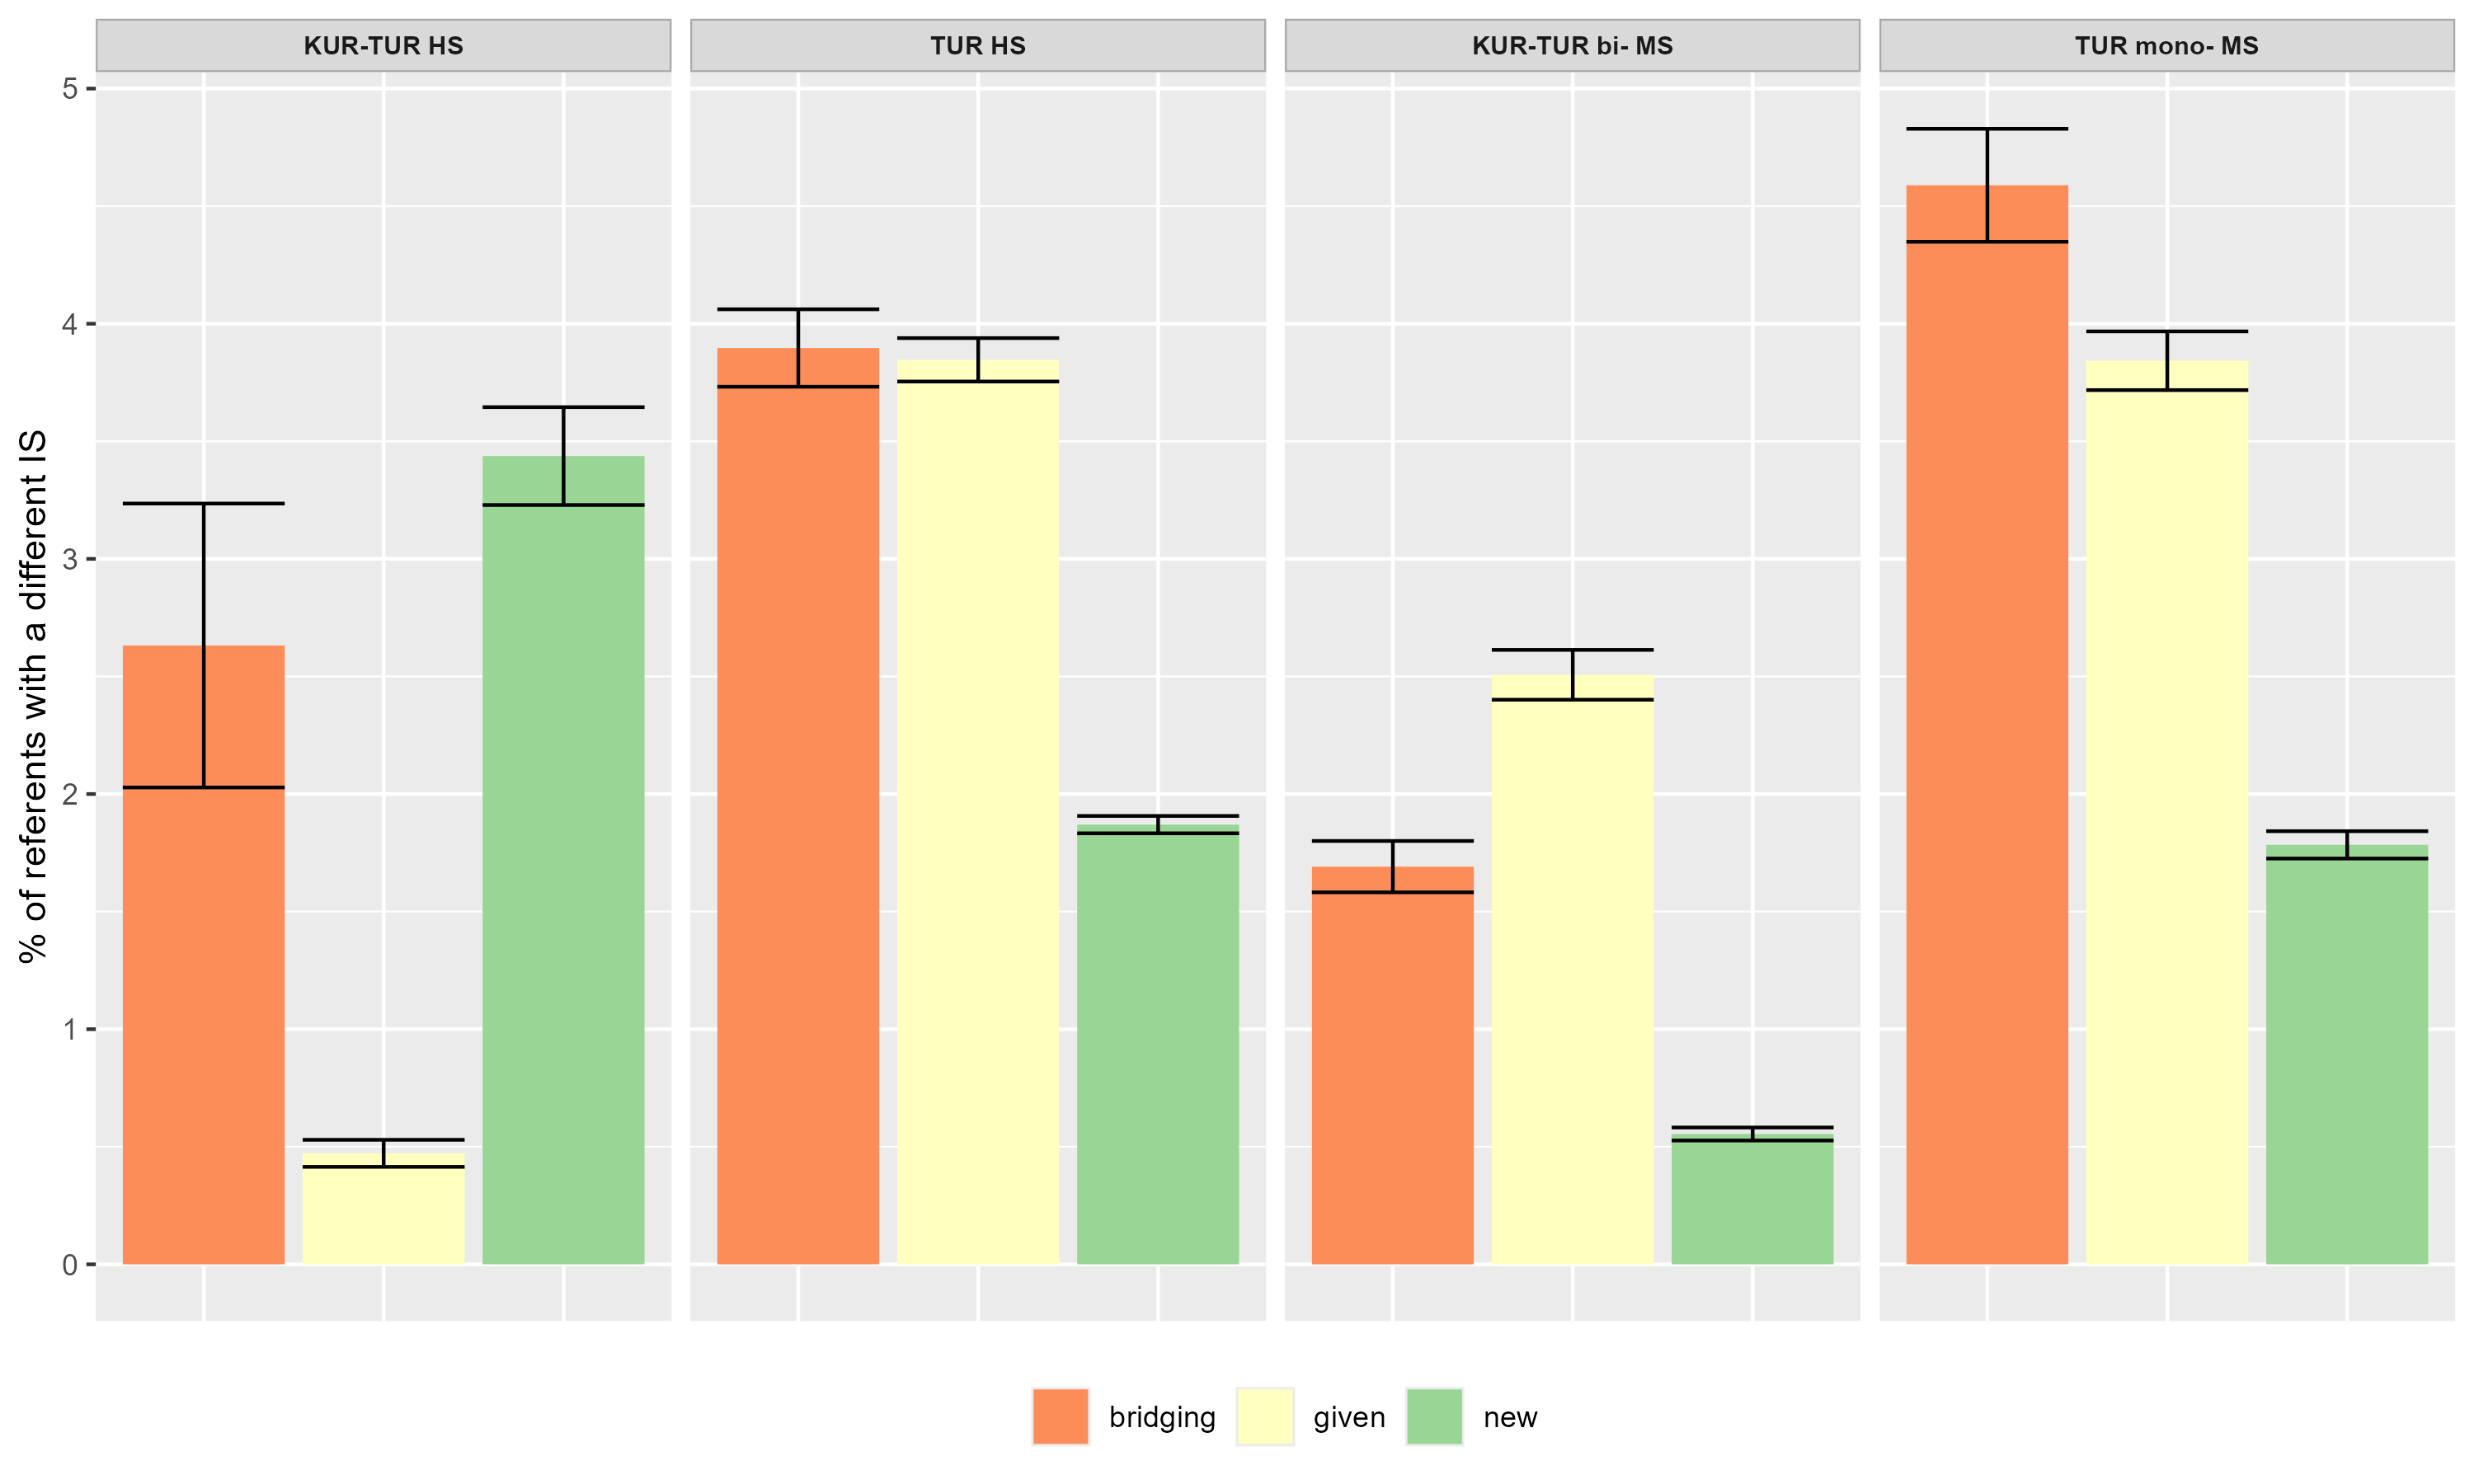
\includegraphics[width=\textwidth]{figures/iefremenko-img011.png}
\caption{\label{fig:key:12}Frequency distribution of referents in the post-predicate position according to their information status.}
\end{figure}

\figref{fig:key:12} illustrates the frequency distribution of referents in the post-predicate position based on their information status in relation to the total number of referents in the texts. Error bars indicate standard error.

The figure reveals that all types of referents appear in the post-predicate position across each group, with bridging and given referents occurring most frequently, except in the trilingual group. Previous research on word order in Turkish indicates that the post-predicate position typically accommodates given or backgrounded information, making the placement of given referents in this position unsurprising. This analysis further reveals that bridging referents—defined as those not explicitly introduced but inferable from the preceding context—also appear in the post-predicate position with a frequency similar to that of given referents. An example of bridging referents is provided in example \REF{ex:key:52}.

\newpage
\ea%52
  \label{ex:key:52} Turkish, TUmo33MT\_isT \\
    \gll iki  tane (--)  insan  yür-üyo  kadın-la  erkek. \\
two  \textsc{clf}    {}  person  walk\textsc{-prs.3sg}  woman\textsc{-inst}  man\\
\glt ‘Two persons are walking, a woman and a man.’   \\
  \z

In the example above, the referents \textit{kadın} ‘woman’ and \textit{erkek} ‘man’ are bridging because they were indirectly introduced as \textit{iki tane insan} ‘two persons’ in the same sentence.

Apart from given and bridging referents, \figref{fig:key:12} shows that speakers across all four groups also placed newly introduced referents in the post-predicate position, despite descriptive grammars of Turkish emphasizing that new information is generally not permitted in this position (\citealt{Kornfilt1997}, \citealt{GokselKerslake2004}). Example \REF{ex:key:53} further illustrates this with a case of a newly introduced referent appearing post-predicatively in the dataset.

\ea%53
  \label{ex:key:53} Turkish, DEbi06FT\_isT \\
     \gll Em (-)  onun  gir-eceğ-i    yer-de    de  böyle    bi\\
 hm  {} his  enter-\textsc{part-poss.3sg}  place-\textsc{loc}  also  like-this  \textsc{art}\\
\gll yan-ın-da     bi  ee  kadın    var-dı    köpeğ-i-yle \\
close\textsc{-poss-loc}  \textsc{art}  hm  woman    be-\textsc{pst.3sg}  dog\textsc{-poss-inst}\\
\glt ‘Hm, at the place where he was entering, so like next to it, there was a woman with her dog.’ \\
  \z

In example \REF{ex:key:53}, the referent \textit{köpeğiyle} ‘with a dog’ is a newly mentioned referent that is not retrievable from the previous context and plays an important role in the further text. As noted earlier, descriptive grammars of Turkish (\citealt{Kornfilt1997}, \citealt{GokselKerslake2004}) state that new information should not appear in the post-predicate position. However, \figref{fig:key:12} shows that speakers of the four groups, including majority Turkish speakers in Turkey, place new referents also in the post-predicate position. The group that employs new referents in the post-predicate position most frequently is Kurmanji-Turkish HS in Germany (\={x}=3.44), followed by HS of Turkish in Germany (\={x}=1.87) and Turkish monolinguals (\={x}=1.78), while the group who places new referents in the post-predicate position least frequently is Kurmanji-Turkish bilinguals in Turkey (\={x}=0.55). However, it is important to note that these occurrences remain relatively rare, with over 95\% of new referents in still appearing in the pre-predicate position. Nevertheless, since the analysis reveals that monolinguals also place new referents in the post-predicate position, bi- or multilingualism alone does not appear to be a determining factor. However, \figref{fig:key:12} suggests that societal status of Turkish may play a role, as heritage speakers place new referents in the post-predicate position more frequently than majority speakers.

To explore the effect of the societal status of Turkish and multilingualism, a linear mixed-effects model was run. The dependent variable was the Percentage of New Referents in the Post-Predicate Position, while the fixed effects included Multilingualism (multilingual vs. monolingual) and Societal Status of Turkish (heritage vs. majority). The variable Participant was included as a random variable to account for individual differences among the speakers. An overview of the regression results is presented in \tabref{tab:key:5.6}.

\begin{table}
\begin{tabularx}{\textwidth}{XYY}
\lsptoprule
\textbf{Random effects:}\\
\midrule
\textbf{Groups} & \textbf{Variance} & \textbf{Standard Deviation}\\
Participant (Intercept) & 0.70 & 0.83\\
Residual & 22.02 & 5.65\\
\midrule
\end{tabularx}
\begin{tabularx}{\textwidth}{Xrrrrr}
% \lsptoprule
\textbf{Fixed effects:}\\
\midrule
\textbf{Fixed effect} & \textbf{Estimate} & \textbf{Std. Error} & \textbf{df}  & \textbf{t-value} & \textbf{\textit{p}-value}\\
(Intercept) & 3.43 & 0.88 & 102.30 & 3.88 & $<.0001^{***}$\\
Multilingualism\\ (multilingual) & -1.23 & 0.75 & 103.04 & -1.62 & 0.10\\
Societal Status\\ (majority) & -1.65 & 0.71 & 103.40 & -2.30 & $.02^{*}$\\
\lspbottomrule
\end{tabularx}

\caption{\label{tab:key:5.6}Regression table for lmer with the dependent variable Percentage of New Referents and the independent variables Multilingualism and Societal Status.}
\end{table}

Multilingualism: Multilingualism is a binary independent variable assigned the levels \textit{multilingual} (HS of Turkish in Germany, HS of Turkish and Kurmanji in Germany, Kurmanji-Turkish bilinguals in Turkey) and \textit{monolingual} (Turkish monolinguals in Turkey) in the study. As seen in \tabref{tab:key:5.6}, there is no effect of multilingualism on the use of new referents in the post-predicate position (estimate: -1.23, SE=0.75, \textit{p} < 0.10).

Societal Status: The societal status of Turkish is a binary independent variable with the levels \textit{majority} (Kurmanji-Turkish bilinguals in Turkey and Turkish monolinguals in Turkey) and \textit{heritage} (HS of Turkish in Germany and HS of Turkish and Kurmanji in Germany). The model shows a negative effect of the majority status (estimate: -1.65, SE=0.71, \textit{p} = .02) on the employment of new referents in the post-predicate position. This means that speakers for whom Turkish is the majority language tend to place fewer new referents in the post-predicate position than heritage speakers of Turkish. In other words, heritage speakers in Germany use the post-predicate position for introducing new referents more frequently than majority speakers in Turkey.

In summary, the model confirmed that the use of new referents in the post-predicate position is not more prevalent among bi- or multilinguals compared to monolinguals. However, it revealed that groups where Turkish is the majority language, such as Kurmanji-Turkish bilinguals and Turkish monolinguals, tend to employ new referents in the post-predicate position less frequently than groups where Turkish is a heritage language. Thus, the results suggest that the loosening of information structural constraints is more likely among heritage speakers of Turkish. Interestingly, among majority speakers in Turkey, monolingual majority speakers use more new referents in the post-predicate position than their bilingual counterparts. This indicates that bilingual majority speakers tend to adhere more closely to canonical structures compared to monolinguals.

To further explore the usage of new referents in the post-predicate position across various communicative situations, the following analysis will examine the impact of formality and mode on their placement.

\begin{figure}[b]
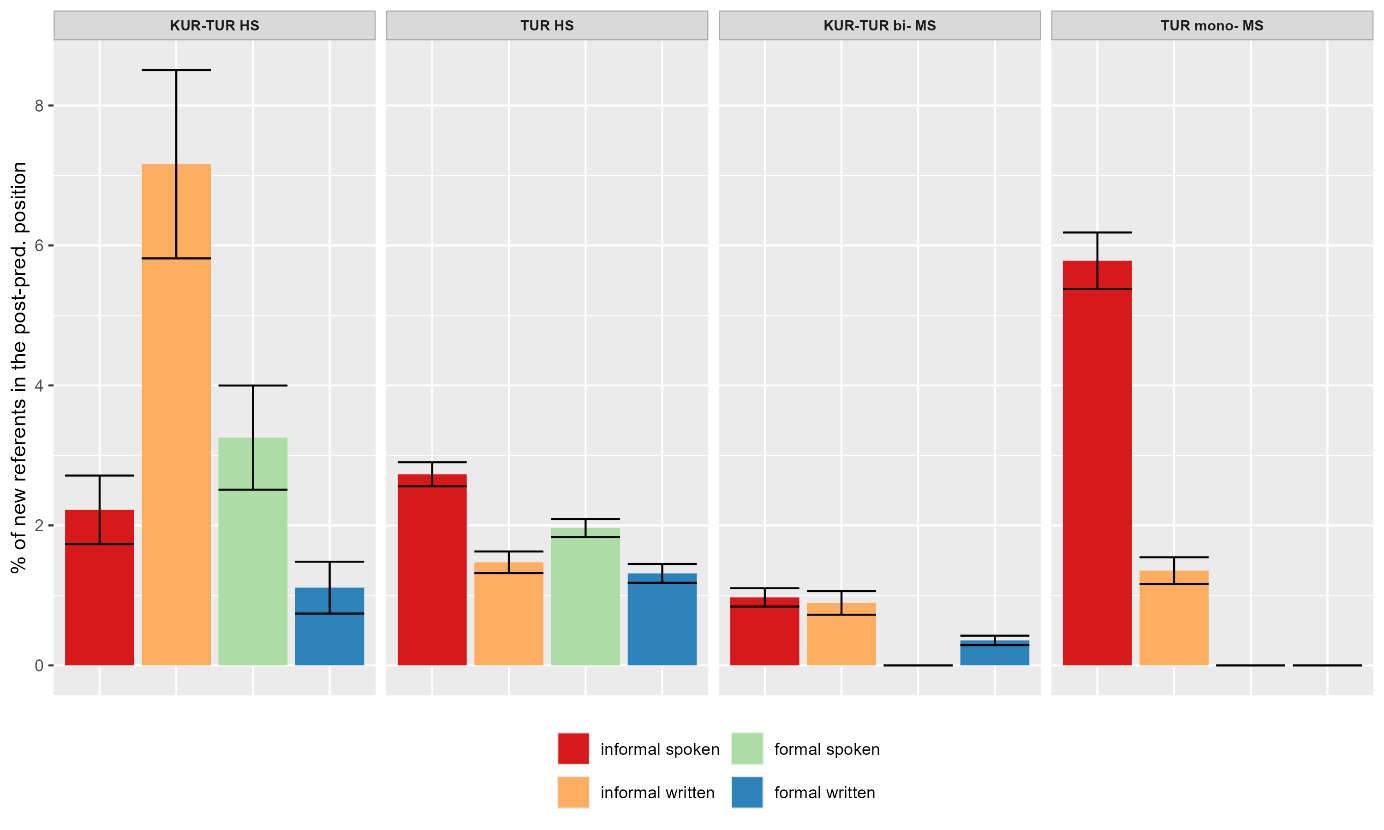
\includegraphics[width=\textwidth]{figures/iefremenko-img012.png}
\caption{\label{fig:key:13}Frequency distribution of new referents across different communicative situations.}
\end{figure}

\largerpage
\figref{fig:key:13} illustrates the frequency distribution of new referents in the post-predicate position relative to the total number of new referents in each communicative situation, with error bars representing standard error. As noted earlier, the absolute number of new referents in the post-predicate position is very low across the speaker groups. Because of this small sample size, the observed distribution should be interpreted with caution. Accordingly, no statistical model is applied, and the discussion is based solely on the patterns visible in the plot.

From \figref{fig:key:13}, it is evident that heritage speakers employ new referents across all communicative situations, while the majority speakers, particularly the monolinguals, predominantly use new referents in the informal situations. This suggests that the higher likelihood of heritage speakers using new referents in the post-predicate position is not solely attributable to the societal status of Turkish, but rather reflects a process of register inflexibility among heritage speakers, where the distinction between formal and informal or spoken and written become less pronounced.

Furthermore, the observation that majority speakers in Turkey, particularly monolinguals, tend to place new information in the post-predicate position challenges the assertions made in descriptive grammars of Turkish, which state that new referents are not permitted in the post-predicate position (\citealt{Erguvanli1984}, \citealt{GokselÖzsoy2000}, \citealt{Issever2003}). However, \citet{DogruozBackus2007} noted that, under certain conditions, focused information can indeed be positioned in the post-predicate position. They argue that focused elements may appear there when “certain linguistic devices, such as discourse markers or the particle \textit{şey}, signal that part of the focus will appear in the postverbal area, or when new information in the postverbal area is less prominent than another piece of focused information in the preverbal area” (\citealt{DogruozBackus2007}: 206).

Following \citet{DogruozBackus2007}, an examination of new referents in the post-predicate position reveals that over half (76\%, n = 35) of these new referents are secondary in relation to nominal referents introduced in the pre-predicate position. For example, in \REF{ex:key:53}, the referent \textit{köpeğiyle} ‘with a dog’ is a new mention, but it is secondary to the preceding referent \textit{bir kadın} ‘a woman.’ In contrast, the remaining 24\% (n=11) of new referents in the post-predicate position were in fact new, as demonstrated in example \REF{ex:key:54}, which features two new referents, \textit{çocuk} ‘a child’ and \textit{bir kadın} ‘a woman,’ both of which are introduced for the first time at the beginning of a narration.

\ea%54
  \label{ex:key:54} Turkish, TUbi26MT\_isT \\
\gll {az  kalsın}  bi  araba  çarp-ıyo-du  çocuk-lu  bi  kadın-a \\
almost \textsc{art}  car  hit-\textsc{prog-pst}  child\textsc{-attr} \textsc{art}  woman\textsc{-dat}\\
\glt ‘A car almost hit a woman with a child.’ \\
  \z

Thus, the analysis indicates that information structural constraints remain intact in Turkish. While new referents can appear in the post-predicate position, they primarily function as secondary elements, often linked to new referents introduced before the predicate.

In summary, the analysis of the information status of referents revealed that all groups include new referents in the post-predicate position, although the number of instances is not high. Furthermore, the majority of these new referents function as ‘less prominent’ elements related to the new referents introduced in the pre-predicate position. Besides, the analysis showed that heritage speakers of Turkish tend to place new referents in the post-predicate position more frequently than the majority speakers, but the differences lie mostly in formal situations. While majority speakers tend to avoid placing new referents in the post-predicate position in formal situations, heritage speakers place them across all communicative situations. Finally, there is also a difference between the majority speakers of Turkish in the data: the monolingual majority speakers tend to employ new referents in the post-predicate position more frequently than the bilingual majority speakers in Turkey. This observation further supports the argument that Kurmanji-Turkish bilinguals in Turkey adhere more closely to canonical language structures than monolingual speakers.

\section{Summary of the findings}\label{sec:key:5.5}

This section discusses the key findings presented in this chapter concerning word order variation in the Turkish varieties. The discussion is structured around three main aspects: (1) different language contact situations with the different intensity this contact, (2) bilingualism and the societal status of Turkish, and (3) the role of register.

The discussion begins by examining the first two factors, focusing on the role of contact languages and the impact of bilingualism and the societal status of Turkish. A quantitative analysis was conducted to calculate the number of post-predicate structures normalized per 100 CUs across the four groups. The results indicate that word order in the investigated speaker groups remains predominantly verb-final: even in the informal spoken situations, where the percentage of post-predicate structures is highest, between 75\% and 85\% of utterances are verb-final. However, it is important to note that there is significant individual variation within the groups: while there are speakers who do not use post-predicate structures in some of their productions at all, others employ this position in more than 60\% of the utterances.

Previous studies on post-predicate structures in Turkish have also found that the word order is predominantly SOV. However, these studies report varying proportions of pre- and post-predicate structures in their data. The documented frequencies of post-predicate structures range from 2\% to 45\% (e.g., \citealt{Antonova-unlu2015, Antonova-unlu2019}, \citealt{DogruozBackus2007}, \citealt{Saginsimsek2016}, \citealt{SchroederEtAl2024}, among others). The differences in the frequency distribution of post-predicate structures across these studies may be attributed to factors such as participants' age, the type of data analyzed (spontaneous vs. elicited), and the level of formality of the analyzed data. In addition, comparisons across studies are complicated by differences in analytical approaches and coding procedures.

The quantitative analysis of post-predicate structures in this study reveals that monolinguals in Turkey use the highest number of such structures. However, Turkish heritage speakers in Germany employ nearly the same frequency of post-predicate structures as the monolinguals, with no significant differences observed between the two groups. Thus, the societal status of Turkish appears to have no impact on the use of post-predicate structures. These findings align with those of \citet{DogruozBackus2007}, who also reported no significant difference in the frequency distribution of post-predicate structures between heritage Turkish in the Netherlands and monolingual Turkish speakers in Turkey.

In contrast, speakers from the two groups where Kurmanji is the contact language use significantly fewer post-predicate structures compared to the monolinguals and Turkish heritage speakers in Germany. This finding suggests that Kurmanji has an influence on Turkish, despite being a heritage language for speakers in both groups.

From the usage-based perspective, frequency is closely related to the entrenchment of a construction, which refers to the degree to which a pattern is recognized as a construction and accessed for productive use. Since Kurmanji is predominantly an SOV language that primarily places goals in the post-predicate position, the entrenchment of verb-final constructions is likely higher than that of post-predicate constructions. This difference may account for the significantly lower number of post-predicate structures in Turkish among Kurmanji speakers compared to those without Kurmanji in their linguistic repertoire.

Additionally, in German, the V2 word order pattern allows for the verb to occupy the second position in main declarative clauses with a finite main verb, which enables any constituent to be placed in the post-predicate position. However, an increase in the use of post-predicate structures among the groups in Germany has not been observed. Therefore, the tendency of the groups in this study to (not) use post-predicate structures cannot be solely attributed to the entrenchment of these constructions in the speakers' minds.

The primary difference between the contact between Turkish and German and Turkish with Kurmanji lies in the intensity of the contact. \citet{ThomasonKaufman1988} define contact intensity as the most significant social factor for predicting contact-induced language change: the more intense the contact, the greater the expected structural changes. \citet{DogruozBackus2007} also highlight the influence of social factors on the degree of borrowability, illustrating this with the example of heritage Turkish in the Netherlands. They argue that due to the relatively recent contact between Turkish and Dutch, heritage Turkish in the Netherlands experiences changes primarily at the construction level, in contrast to Gagauz, which has reached a stage of syntactic borrowing.

Similarly, the frequency analysis in this study shows that the groups with Kurmanji as the contact language employ fewer post-predicate structures than the groups where Kurmanji is not the contact language. These results indicate that the intensity of contact plays a crucial role in determining changes in the post-predicate domain. However, unlike Gagauz, Turkish in contact with Kurmanji in this study adheres to the unmarked SOV word order in Turkish. Yet, as demonstrated later on, the intensity of contact is not the only factor driving the observed changes.

In addition to the frequency differences between the groups, the analysis of the composition types of post-predicate structures—focusing on weight, types, and semantic roles—revealed no evidence of convergence in the post-predicate domain in Turkish. It was anticipated that the bilingual and trilingual groups, where Turkish is in contact with German and/or Kurmanji, would place nominal constituents in the post-predicate position more frequently than the groups in Turkey. However, the analysis indicated that Turkish monolinguals actually use the highest number of nominal constituents in the post-predicate position.

Furthermore, it was expected that the groups with Kurmanji as the contact language would exhibit a higher frequency of goals of motion, addressees, and recipients in the post-predicate position within their Turkish compared to the groups without Kurmanji in their repertoire. Contrary to this expectation, the analysis again revealed that Turkish monolinguals have the highest occurrence of goals of motion in the post-predicate position. This point will be revisited in \sectref{sec:key:7.2}.

In summary, the analysis revealed a quantitative difference in the frequency distribution of post-predicate structures between groups with and without Kurmanji in their repertoire, suggesting a potential CLI from Kurmanji to Turkish.

The third factor examined the impact of communicative situations on the use of post-predicate structures. As outlined in \sectref{sec:key:3.1.1}, the post-predicate position in Turkish is primarily employed in informal situations and spoken modes, with normative pressure discouraging its use in formal settings (\citealt{Erguvanli1984, Schroeder1995}). Overall, the frequency distribution of post-predicate structures in various communicative situations displays a similar pattern across the groups: the highest number of post-predicate structures occurs in informal spoken contexts, followed by informal written and formal spoken situations, while the lowest frequency is observed in formal written contexts.

The model revealed that while formality and mode significantly influence the use of post-predicate structures in Turkish monolinguals and Turkish HS in Germany, formality does not affect their use in Turkish bilingual speakers in Turkey or Kurmanji-Turkish HS in Germany. Similarly, while mode impacts the frequency of post-predicate structures in Turkish bilingual speakers in Turkey, it has no significant effect on Kurmanji-Turkish HS in Germany. These findings suggest that Turkish monolinguals and Turkish HS in Germany differentiate clearly between communicative situations, whereas Turkish bilingual speakers in Turkey show no notable variation based on formality, and Kurmanji-Turkish HS in Germany display no significant differences based on either formality or mode.

Heritage speakers are typically exposed to predominantly informal registers in their heritage language, often leading to register inflexibility across various linguistic phenomena (see \citealt{WieseEtAl2022}, \citealt{AlexiadouRizou2023}, \citealt{OzsoyEtAl2022}). Using the same methodology as in the current study, \citet{SchroederEtAl2024} found evidence of register inflexibility in Turkish heritage speakers in the U.S., where post-predicate structures were used at nearly the same frequency in both formal and informal settings. However, the analysis of Turkish heritage speakers in Germany in this study revealed a different pattern: while no register inflexibility was observed among Turkish HS in Germany, Kurmanji-Turkish HS showed no significant differences in the use of post-predicate structures based on either formality or mode. However, given the small sample size of the trilingual dataset (nine speakers), these findings should be interpreted with caution.

Furthermore, unlike monolingual majority speakers in Turkey, Turkish bilingual speakers in Turkey show no notable variation in the use of post-predicate structures based on formality. This difference is particularly noteworthy. Two possible explanations may account for these group differences. First, Kurmanji speakers are largely exposed to Turkish in formal situations, where verb-final word order is predominant. As a result, the preverbal construction becomes highly entrenched due to the unmarked SOV word order in both Kurmanji and formal Turkish. Second, the avoidance of post-predicate structures in informal situations by Kurmanji speakers may stem from a broader tendency among bilinguals to use canonical language forms when speaking their majority language, even in informal settings. This behavior is influenced by standard language ideology and biased attitudes toward bilinguals (\citealt{SevincDewaele2018}, \citealt{Bunk2024, bunk_anxious_2025}). These two explanations will be explored further in \sectref{sec:key:7.3}.

Beyond the frequency of post-predicate structures, this chapter examined their use with a focus on the information status of referents. As discussed in Chapter 2, Turkish word order is shaped by information structural requirements, placing background information in the post-predicate position while restricting new information after the predicate (\citealt{Erguvanli1984, Issever2003}). Consequently, the use of the post-predicate position operates at the syntax-discourse/pragmatics interface.

In bilingualism, second language acquisition, and language contact research, structural changes are often found at the interface between syntax and pragmatics/semantics \citep{Sorace2011}. In the case of Turkish, word order is strongly influenced by information structure, with topics typically sentence-initial, foci immediately pre-predicate, and background (given) information in the post-predicate position (\citealt{Erguvanli1984, Issever2003}). Because information structure governs the mapping of discourse-related features onto syntactic positions, it constitutes a phenomenon at the external syntax-pragmatics interface. Studies on heritage languages (\citealt{MontrulPolinsky2011}, \citealt{PascualEtAl2012}) suggest that external interfaces are more vulnerable than internal ones in heritage speakers. However, other studies (e.g., \citealt{Gondra2022, martynova2024ov}) challenge this claim, finding no evidence of external interface vulnerability. Therefore, this chapter addressed how information structural constraints at the external syntax-pragmatics interface affect the use of the post-predicate position in Turkish under conditions of language contact.

The analysis of Turkish word order from an information structure perspective revealed that speakers across all four groups, including monolinguals, frequently place new referents in the post-predicate position. This suggests that bilingualism and contact languages do not have an effect on the employment of new referents in the post-predicate position. This finding contradicts traditional descriptive grammars of Turkish, which assert that the post-predicate position is reserved for background information (\citealt{Erguvanli1984}, \citealt{GokselÖzsoy2000}, \citealt{Issever2003}). However, \citet{DogruozBackus2007} demonstrated that under certain conditions, Turkish allows new information in the post-predicate position—particularly when it is less prominent than other new information in the pre-predicate position. The current study supports this observation, showing that most new referents in the post-predicate position convey secondary information about a referent introduced in the pre-predicate position.

Although all groups place new referents in the post-predicate position, the analysis indicates that Turkish as a heritage language positively influences this tendency. Bilingual and trilingual heritage speakers in Germany place new referents post-predicatively more frequently than majority Turkish speakers. However, the analysis of frequency distribution across different communicative situations revealed that while majority Turkish speakers primarily use new referents in informal situations, heritage speakers employ them in both informal and formal contexts. These findings suggest a spread of informal features into formal registers rather than a vulnerability of grammatical features at the syntax-pragmatics interface in heritage speakers. The issue of register inflexibility will be revisited in \sectref{sec:key:7.3}.

Furthermore, the analysis of new referent placement shows that Kurmanji-Turkish bilinguals use fewer new referents in the post-predicate position than Turkish monolinguals. The distinction between the two groups of majority Turkish speakers in Turkey supports the conclusion that bilingualism does not drive changes at the external interface in this study. Moreover, the results further highlight the tendency of Kurmanji-Turkish bilinguals to favor more canonical structures than monolinguals. The implications of these findings for monolingual majority Turkish speakers will be explored in \sectref{sec:key:7.2}.

To summarize the findings on Turkish, the analysis revealed no quantitative differences between majority and heritage speakers in their use of the post-predicate position, either overall or across different communicative situations. Instead, heritage speakers of Turkish in Germany align with monolingual majority speakers in Turkey, while Kurmanji-Turkish heritage speakers in Germany resemble bilingual majority speakers in Turkey. The key distinction lies between speakers with and without Kurmanji in their repertoire: those with Kurmanji use fewer post-predicate structures than those without Kurmanji in their repertoire, and this difference seems to be driven by the different use of this position across communicative situations.

Although no quantitative differences in the frequency of post-predicate structures emerged between majority and heritage speakers, the analysis of referent information status revealed that heritage speakers more frequently place new referents in the post-predicate position than majority speakers. This pattern reflects the spread of informal linguistic features into formal registers among heritage speakers. As for the bilingual majority speakers in Turkey, the analysis of information status corroborated the claim that bilingual majority speakers favor more canonical structures than monolinguals, as evidenced by their lower use of new referents in the post-predicate position.

